%% Volume I, Chapter 17: Determinants
\chapter{Determinants}
\label{ch:determinants}

\abstract{A square matrix stretches space, and a single number says by how much: the factor by which it multiplies every volume, with a sign that records whether it turns space inside out. This number, the determinant, vanishes exactly when the matrix cannot be undone, and it is the factor that appears whenever the variables of an integral are changed. Its defining formula has one term for every rearrangement of the columns, far too many to add up even for moderate sizes, yet elimination produces the same number with a few multiples of $n^3$ operations. Why the two descriptions agree, and why the number must be handled with care in floating-point arithmetic, is the story of this chapter.}

Determinants have been with us for several chapters, always as a promise. \Cref{prop:inverse-2x2} found that a $2\times2$ matrix is invertible exactly when the number $ad-bc$ is nonzero, and \cref{thm:invertible-matrices} stated the corresponding facts for $n\times n$ matrices without proof. \Cref{thm:linear-volume} showed that a linear map multiplies volumes by $|\det A|$, but for $n>2$ it borrowed two facts about determinants, the product rule and the determinants of the elementary matrices. The triple product of \cref{prop:cross-product}, the Schur complement of \cref{thm:schur-complement}, the factorisation $PA=LU$ of \cref{thm:plu}, the Wronskian of \cref{sec:independence}, the minors of \cref{thm:rank-characterisations} and the invariants of similar matrices in \cref{prop:similarity-invariants} all pointed forward to this chapter. Here the debts are paid.

The approach is to characterise the determinant before computing it. The signed area of a parallelogram, regarded as a function of its two sides, is linear in each side, changes sign when the sides are exchanged, and gives $1$ for the unit square. We shall see that in every dimension there is exactly one function of $n$ vectors with the corresponding three properties, and that it is given by a sum over all permutations. Almost every property of the determinant, the product rule among them, then follows from this uniqueness in a few lines, without computation. The sum over permutations requires the sign of a permutation, which \cref{ch:sets,ch:counting} did not define; \cref{sec:permutations-signs} supplies it.

As in \cref{ch:vector-spaces,ch:linear-maps}, $\mathbb F$ denotes $\mathbb R$ or $\mathbb C$, and the algebraic results hold for both with the same proofs; the results about volume, orientation and Gram matrices are stated for real matrices. Eigenvalues, the subject of \cref{ch:eigenvalues}, and orthonormal bases and the QR factorisation, the subject of \cref{ch:inner-products}, are not used, and we indicate where they will connect with determinants. Every result of the chapter is proved.

The chapter is organised as follows. \Cref{sec:det-geometry} looks at signed areas and volumes in the plane and in space and extracts the properties that will define the determinant. \Cref{sec:permutations-signs} defines the sign of a permutation and proves that it is multiplicative. \Cref{sec:det-definition} proves that exactly one function has the defining properties and gives the formula for it, and \cref{sec:det-properties} derives its main properties: the rules for transposes, row operations and products, and the criterion for invertibility. \Cref{sec:det-elimination} computes determinants by elimination, and \cref{sec:cofactor} develops the expansion by cofactors, the adjugate matrix and Cramer's rule. \Cref{sec:det-block} treats block matrices and low-rank updates, \cref{sec:det-volume} returns to volume, orientation and the Gram determinant, and \cref{sec:minors-functions} relates minors to the rank and differentiates determinants. \Cref{sec:det-computation} looks at determinants in floating-point arithmetic.

\section{Area, Volume, and Orientation}
\label{sec:det-geometry}

\subsection{Signed Area in the Plane}

Two vectors $\mathbf u=(u_1,u_2)$ and $\mathbf v=(v_1,v_2)$ of the plane span the parallelogram
\[
P(\mathbf u,\mathbf v)\coloneqq\{s\mathbf u+t\mathbf v: 0\le s,t\le1\},
\]
the image of the unit square under the matrix with the columns $\mathbf u$ and $\mathbf v$. By \cref{thm:linear-volume}, whose proof for $n=2$ is complete, its area is $|u_1v_2-u_2v_1|$. We want to understand this number as a function of the two vectors, and to find properties that single it out, because these properties will make sense in every dimension.

The area itself is not a convenient function: replacing $\mathbf u$ by $-\mathbf u$ does not change the parallelogram's area, so the area is not linear in $\mathbf u$. The remedy is to give the area a sign. We say that the pair $(\mathbf u,\mathbf v)$ is \emph{positively oriented} if $\mathbf v$ lies on the left of the line through $\mathbf u$, seen from the origin in the direction of $\mathbf u$, so that $\mathbf u$ is turned towards $\mathbf v$ counterclockwise through an angle less than $\pi$, and \emph{negatively oriented} if $\mathbf v$ lies on the right. The \term{signed area} $\mathcal A(\mathbf u,\mathbf v)$ is the area of $P(\mathbf u,\mathbf v)$ with the sign $+$ in the first case, the sign $-$ in the second, and $0$ if the parallelogram degenerates to a segment or a point.

The signed area is easy to compute as base times signed height. Let $\mathbf u\ne\mathbf 0$, and let $\mathbf n\coloneqq(-u_2,u_1)/\|\mathbf u\|$ be the unit vector obtained by turning $\mathbf u/\|\mathbf u\|$ counterclockwise through a right angle. The distance of $\mathbf v$ from the line through $\mathbf u$ is $|\langle\mathbf n,\mathbf v\rangle|$, and $\langle\mathbf n,\mathbf v\rangle$ is positive exactly when $\mathbf v$ lies on the left of that line, on the side into which $\mathbf n$ points (\cref{fig:signed-area}A). The base of the parallelogram has the length $\|\mathbf u\|$, so
\begin{equation}
\mathcal A(\mathbf u,\mathbf v)=\|\mathbf u\|\,\langle\mathbf n,\mathbf v\rangle=-u_2v_1+u_1v_2=u_1v_2-u_2v_1 .
\label{eq:signed-area}
\end{equation}
This is the number $\mathbf u\wedge\mathbf v$ that \cref{sec:vector-numerics} used to decide on which side of an edge a point lies, and the determinant $ad-bc$ of \cref{prop:inverse-2x2} for the matrix with the columns $\mathbf u=(a,c)$ and $\mathbf v=(b,d)$.

\begin{figure}
\sdpanel{A}{\begin{tikzpicture}[scale=1.15, font=\scriptsize]
\fill[sdfill] (0,0) -- (2,0.6) -- (2.7,2.1) -- (0.7,1.5) -- cycle;
\draw[line width=0.6pt] (0,0) -- (2,0.6) -- (2.7,2.1) -- (0.7,1.5) -- cycle;
\draw[black!60, dashed, line width=0.5pt] (-0.3,-0.09) -- (2.6,0.78);
\draw[densely dotted, line width=0.6pt] (1.055,0.3165) -- (0.7,1.5);
\node[right] at (0.83,0.95) {$h$};
\draw[line width=0.9pt, -{Latex[length=1.8mm]}] (0,0) -- (2,0.6) node[below right=-1pt] {$\mathbf u$};
\draw[line width=0.9pt, -{Latex[length=1.8mm]}] (0,0) -- (0.7,1.5) node[left] {$\mathbf v$};
\draw[line width=0.6pt, -{Latex[length=1.5mm]}] (1.6,0.48) -- (1.4126,1.1046) node[above] {$\mathbf n$};
\end{tikzpicture}}\hfill
\sdpanel{B}{\begin{tikzpicture}[scale=1.15, font=\scriptsize]
\fill[sdfill] (0,0) -- (2,0) -- (2.4,1.2) -- (0.4,1.2) -- cycle;
\draw[line width=0.6pt] (0,0) -- (2,0) -- (2.4,1.2) -- (0.4,1.2) -- cycle;
\draw[dashed, line width=0.6pt] (0,0) -- (2,0) -- (3.6,1.2) -- (1.6,1.2) -- cycle;
\draw[black!60, densely dotted, line width=0.5pt] (-0.2,1.2) -- (3.8,1.2);
\draw[line width=0.9pt, -{Latex[length=1.8mm]}] (0,0) -- (2,0) node[below] {$\mathbf u$};
\draw[line width=0.9pt, -{Latex[length=1.8mm]}] (0,0) -- (0.4,1.2) node[above left=-1pt] {$\mathbf v$};
\draw[line width=0.9pt, -{Latex[length=1.8mm]}] (0,0) -- (1.6,1.2) node[above] {$\mathbf v+t\mathbf u$};
\end{tikzpicture}}\hfill
\sdpanel{C}{\begin{tikzpicture}[scale=1.15, font=\scriptsize]
\fill[sdfill] (0,0) -- (2,0) -- (2.3,0.8) -- (0.3,0.8) -- cycle;
\fill[black!25] (0.3,0.8) -- (2.3,0.8) -- (2.9,1.5) -- (0.9,1.5) -- cycle;
\draw[line width=0.6pt] (0,0) -- (2,0) -- (2.3,0.8) -- (0.3,0.8) -- cycle;
\draw[line width=0.6pt] (0.3,0.8) -- (2.3,0.8) -- (2.9,1.5) -- (0.9,1.5) -- cycle;
\draw[dashed, line width=0.6pt] (0,0) -- (0.9,1.5) (2,0) -- (2.9,1.5);
\draw[line width=0.9pt, -{Latex[length=1.8mm]}] (0,0) -- (2,0) node[below] {$\mathbf u$};
\draw[line width=0.9pt, -{Latex[length=1.8mm]}] (0,0) -- (0.3,0.8) node[left] {$\mathbf v$};
\draw[line width=0.9pt, -{Latex[length=1.8mm]}] (0.3,0.8) -- (0.9,1.5) node[left] {$\mathbf w$};
\end{tikzpicture}}
\caption{Three properties of the signed area. (A) The parallelogram spanned by $\mathbf u=(2,0.6)$ and $\mathbf v=(0.7,1.5)$ has the base $\|\mathbf u\|$ and the height $h=\langle\mathbf n,\mathbf v\rangle$, where $\mathbf n$ is the unit normal on the left of $\mathbf u$; its signed area is $2\cdot1.5-0.6\cdot0.7=2.58$. (B) A shear: $\mathbf v$ and $\mathbf v+t\mathbf u$ (here $t=0.6$) have the same height above the line through $\mathbf u$, so the two parallelograms (shaded and dashed) have the same area. (C) Additivity: the heights of $\mathbf v$ and $\mathbf w$ over the base $\mathbf u$ add up to the height of $\mathbf v+\mathbf w$, and the two shaded parallelograms together have the area of the parallelogram spanned by $\mathbf u$ and $\mathbf v+\mathbf w$, whose sides are dashed.}
\label{fig:signed-area}
\end{figure}

Formula \eqref{eq:signed-area} shows the properties of the signed area at once, and \cref{fig:signed-area} shows their geometric meaning.
\begin{enumerate}
\item \emph{Linearity in each vector.} For fixed $\mathbf u$, the signed height $\langle\mathbf n,\mathbf v\rangle$ is a linear function of $\mathbf v$, so $\mathcal A(\mathbf u,s\mathbf v+t\mathbf w)=s\,\mathcal A(\mathbf u,\mathbf v)+t\,\mathcal A(\mathbf u,\mathbf w)$. Geometrically, heights over a fixed base add (panel C), and stretching one side stretches the area by the same factor, with a change of sign if the factor is negative. By symmetry of the formula, $\mathcal A$ is linear in $\mathbf u$ as well.
\item \emph{Alternation.} $\mathcal A(\mathbf u,\mathbf u)=0$, since a parallelogram with two equal sides is flat, and $\mathcal A(\mathbf v,\mathbf u)=-\mathcal A(\mathbf u,\mathbf v)$, since exchanging the sides reverses the orientation.
\item \emph{Normalisation.} $\mathcal A(\mathbf e_1,\mathbf e_2)=1$: the unit square has area $1$, and $\mathbf e_2$ lies on the left of $\mathbf e_1$.
\end{enumerate}
A consequence of the first two properties is the invariance under shears in panel B: $\mathcal A(\mathbf u,\mathbf v+t\mathbf u)=\mathcal A(\mathbf u,\mathbf v)+t\,\mathcal A(\mathbf u,\mathbf u)=\mathcal A(\mathbf u,\mathbf v)$. Sliding the top side of a parallelogram along itself changes neither the base nor the height.

The three properties determine the signed area completely, and the argument that shows this is the model for everything in \cref{sec:det-definition}. Write $\mathbf u=u_1\mathbf e_1+u_2\mathbf e_2$ and $\mathbf v=v_1\mathbf e_1+v_2\mathbf e_2$, and expand by linearity in each vector:
\[
\mathcal A(\mathbf u,\mathbf v)=u_1v_1\,\mathcal A(\mathbf e_1,\mathbf e_1)+u_1v_2\,\mathcal A(\mathbf e_1,\mathbf e_2)+u_2v_1\,\mathcal A(\mathbf e_2,\mathbf e_1)+u_2v_2\,\mathcal A(\mathbf e_2,\mathbf e_2).
\]
By alternation the first and the last term vanish and $\mathcal A(\mathbf e_2,\mathbf e_1)=-\mathcal A(\mathbf e_1,\mathbf e_2)$, and by normalisation $\mathcal A(\mathbf e_1,\mathbf e_2)=1$; so $\mathcal A(\mathbf u,\mathbf v)=u_1v_2-u_2v_1$. Any function of two plane vectors with the three properties must be this one. Of the four products $u_iv_j$, those with $i=j$ are killed by alternation, and the two others survive with the signs of the two arrangements $(\mathbf e_1,\mathbf e_2)$ and $(\mathbf e_2,\mathbf e_1)$ of the basis vectors.

\subsection{Volume in Space and the Triple Product}

Three vectors $\mathbf a_1,\mathbf a_2,\mathbf a_3$ of $\mathbb R^3$ span the parallelepiped $P(\mathbf a_1,\mathbf a_2,\mathbf a_3)$ of all combinations $t_1\mathbf a_1+t_2\mathbf a_2+t_3\mathbf a_3$ with $0\le t_i\le1$. Its volume is the area of the base $P(\mathbf a_1,\mathbf a_2)$ times the height of $\mathbf a_3$ above the plane of the base, a familiar rule that \cref{thm:cavalieri} justifies, since the sections parallel to the base are translates of it. By \cref{prop:cross-product}, the cross product $\mathbf a_1\times\mathbf a_2$ is perpendicular to the base and has the length of its area. If the base is not flat, $\mathbf n\coloneqq\mathbf a_1\times\mathbf a_2/\|\mathbf a_1\times\mathbf a_2\|$ is a unit normal, the height is $|\langle\mathbf n,\mathbf a_3\rangle|$ (\cref{fig:parallelepiped}), and
\[
\operatorname{vol}P(\mathbf a_1,\mathbf a_2,\mathbf a_3)=\|\mathbf a_1\times\mathbf a_2\|\,|\langle\mathbf n,\mathbf a_3\rangle|=\bigl|\langle\mathbf a_1\times\mathbf a_2,\mathbf a_3\rangle\bigr| .
\]
Without the absolute value, the triple product $\langle\mathbf a_1\times\mathbf a_2,\mathbf a_3\rangle$ is a \emph{signed volume}: positive when $\mathbf a_3$ lies on the same side of the base as $\mathbf a_1\times\mathbf a_2$, that is, when $(\mathbf a_1,\mathbf a_2,\mathbf a_3)$ is a right-handed triple like $(\mathbf e_1,\mathbf e_2,\mathbf e_3)$, and negative for a left-handed triple. It has the three properties of the signed area: it is linear in each vector, by \cref{prop:cross-product}\,(i) and the linearity of the inner product; it vanishes when two vectors are equal, since $\mathbf a_1\times\mathbf a_1=\mathbf 0$ and $\mathbf a_1\times\mathbf a_2$ is orthogonal to $\mathbf a_1$ and to $\mathbf a_2$; and $\langle\mathbf e_1\times\mathbf e_2,\mathbf e_3\rangle=\langle\mathbf e_3,\mathbf e_3\rangle=1$. \Cref{prop:triple-product} shows that it is the $3\times3$ determinant of \cref{sec:vectors-rn}, as \cref{prop:cross-product}\,(ii) found by expanding both sides.

\begin{figure}
\sdfloat{%
\begin{tikzpicture}[x={(-0.45cm,-0.6cm)}, y={(1.3cm,0cm)}, z={(0cm,1.3cm)}, font=\scriptsize]
\fill[sdfill] (0,0,0) -- (1.6,0.4,0) -- (1.6,2.4,0) -- (0,2,0) -- cycle;
\draw[line width=0.6pt] (0,0,0) -- (1.6,0.4,0) -- (1.6,2.4,0) -- (0,2,0) -- cycle;
\draw[line width=0.6pt] (0.3,0.5,1.4) -- (1.9,0.9,1.4) -- (1.9,2.9,1.4) -- (0.3,2.5,1.4) -- cycle;
\draw[line width=0.6pt] (1.6,0.4,0) -- (1.9,0.9,1.4) (1.6,2.4,0) -- (1.9,2.9,1.4) (0,2,0) -- (0.3,2.5,1.4);
\draw[densely dotted, line width=0.7pt] (0.3,0.5,1.4) -- (0.3,0.5,0);
\fill (0.3,0.5,0) circle (0.9pt);
\node[right] at (0.3,0.5,0.4) {$h$};
\draw[line width=0.9pt, -{Latex[length=1.8mm]}] (0,0,0) -- (1.6,0.4,0) node[below] {$\mathbf a_1$};
\draw[line width=0.9pt, -{Latex[length=1.8mm]}] (0,0,0) -- (0,2,0) node[below right=0pt] {$\mathbf a_2$};
\draw[line width=0.9pt, -{Latex[length=1.8mm]}] (0,0,0) -- (0.3,0.5,1.4) node[above left=-1pt] {$\mathbf a_3$};
\draw[line width=0.6pt, -{Latex[length=1.6mm]}] (0.8,1.4,0) -- (0.8,1.4,1.0) node[pos=0.75, right] {$\mathbf a_1\times\mathbf a_2$};
\end{tikzpicture}}{The parallelepiped spanned by $\mathbf a_1=(1.6,0.4,0)$, $\mathbf a_2=(0,2,0)$ and $\mathbf a_3=(0.3,0.5,1.4)$. The base $P(\mathbf a_1,\mathbf a_2)$ (shaded) lies in the plane $z=0$ and has the area $\|\mathbf a_1\times\mathbf a_2\|=3.2$; the cross product points upwards, and the height of $\mathbf a_3$ above the base is $h=1.4$ (dotted). The signed volume $\langle\mathbf a_1\times\mathbf a_2,\mathbf a_3\rangle=3.2\cdot1.4=4.48$ is positive: the triple is right-handed.\label{fig:parallelepiped}}
\end{figure}

\subsection{The Programme for \texorpdfstring{$n$}{n} Dimensions}

In $\mathbb R^n$ we do not have a cross product, nor, as yet, a rigorous notion of height above a hyperplane. What survives in every dimension are the three properties: a \emph{signed volume} of the parallelepiped spanned by $n$ vectors should be linear in each vector, should vanish when two of the vectors coincide, and should be $1$ for the unit cube. The rest of the chapter carries out this programme. \Cref{sec:det-definition} shows that exactly one function of $n$ vectors in $\mathbb F^n$ has the three properties, the determinant, and \cref{sec:det-volume} proves that its absolute value is the volume of the parallelepiped in the sense of \cref{ch:multiple-integrals}. The expansion that settled the case $n=2$ will be repeated with $n$ vectors, and the surviving terms will correspond to the arrangements of the basis vectors, that is, to permutations; we first need to know how to give a permutation a sign.

\section{Permutations and Signs}
\label{sec:permutations-signs}

\subsection{Permutations, Cycles and Transpositions}

A permutation of $\{1,\ldots,n\}$ is a bijection of this set onto itself (\cref{sec:injections}), and by \cref{thm:arrangements} there are $n!$ of them. We denote the set of all permutations of $\{1,\ldots,n\}$ by $S_n$. Permutations are composed as functions, $\sigma\tau\coloneqq\sigma\circ\tau$, first $\tau$, then $\sigma$; the composition of two permutations is a permutation, the composition is associative, the identity $\operatorname{id}$ is a permutation, and every permutation has an inverse that is again a permutation (\cref{sec:injections}). A set with an operation of this kind is called a \term{group}, and $S_n$ is the \term{symmetric group} of degree $n$; for $n\ge3$ it is not commutative. For small $n$ we write a permutation in \term{one-line notation} as the list of its values $\sigma(1)\sigma(2)\cdots\sigma(n)$; thus $\sigma=3142$ is the permutation with $\sigma(1)=3$, $\sigma(2)=1$, $\sigma(3)=4$ and $\sigma(4)=2$.

Two kinds of permutations are basic. For distinct $a_1,\ldots,a_k$ in $\{1,\ldots,n\}$, the \term{cycle} $(a_1\,a_2\,\cdots\,a_k)$ is the permutation that maps $a_1\mapsto a_2\mapsto\cdots\mapsto a_k\mapsto a_1$ and fixes every other element; $k$ is its \term{length}. A cycle of length $2$, $(a\,b)$, exchanges $a$ and $b$ and is called a \term{transposition}. The permutation $3142$ maps $1\mapsto3\mapsto4\mapsto2\mapsto1$, so it is the cycle $(1\,3\,4\,2)$ of length $4$. Two cycles are \term{disjoint} if they move no common element; disjoint cycles commute, since each acts only on elements that the other fixes.

\begin{proposition}[Cycles and transpositions]
\label{prop:cycles}
Let $\sigma\in S_n$.
\begin{enumerate}
\item $\sigma$ is a product of disjoint cycles, one for each orbit $\{a,\sigma(a),\sigma^2(a),\ldots\}$ of $\sigma$; if the fixed points are counted as cycles of length $1$, the number $c(\sigma)$ of cycles is determined by $\sigma$.
\item A cycle of length $k$ is a product of $k-1$ transpositions: $(a_1\,a_2\,\cdots\,a_k)=(a_1\,a_2)(a_2\,a_3)\cdots(a_{k-1}\,a_k)$.
\item Consequently $\sigma$ is a product of $n-c(\sigma)$ transpositions. In particular, every permutation is a product of transpositions, and the identity is the empty product.
\end{enumerate}
\end{proposition}

\begin{proof}
(i) For $a\in\{1,\ldots,n\}$, the elements $a,\sigma(a),\sigma^2(a),\ldots$ cannot all be distinct, so there is a first repetition $\sigma^i(a)=\sigma^j(a)$ with $i<j$; applying $\sigma^{-1}$ $i$ times gives $a=\sigma^{j-i}(a)$, so $i=0$, and the sequence runs through $k\coloneqq j$ distinct elements and returns to $a$. On this orbit, $\sigma$ acts as the cycle $(a\,\sigma(a)\,\cdots\,\sigma^{k-1}(a))$. Two orbits are either equal or disjoint, since each is the orbit of any of its elements, so the orbits partition $\{1,\ldots,n\}$, and $\sigma$ is the product of the cycles on its orbits, which are disjoint. The orbits depend only on $\sigma$, and so does their number. (ii) We follow an element through the product from the right. The transposition $(a_{k-1}\,a_k)$ maps $a_{k-1}$ to $a_k$, which the other factors fix, so $a_{k-1}\mapsto a_k$. For $i<k-1$, the factors to the right of $(a_i\,a_{i+1})$ fix $a_i$, the factor $(a_i\,a_{i+1})$ maps it to $a_{i+1}$, and the factors to the left fix $a_{i+1}$; so $a_i\mapsto a_{i+1}$. Finally $a_k$ is moved to $a_{k-1}$ by the last factor, then to $a_{k-2}$, and so on, until the first factor maps $a_2$ to $a_1$; so $a_k\mapsto a_1$. Elements other than the $a_i$ are fixed. (iii) A cycle of length $k$ contributes $k-1$ transpositions, and the lengths of the cycles add up to $n$; so the number of transpositions is $\sum(k_i-1)=n-c(\sigma)$.
\end{proof}

The decomposition into transpositions is far from unique: $(1\,2)(1\,2)=\operatorname{id}$, and $(1\,2\,3)=(1\,2)(2\,3)=(2\,3)(1\,3)$, as one checks by following the three elements. What is unique, as we now show, is whether the number of transpositions is even or odd.

\subsection{Inversions and the Sign}

\begin{definition}[Inversions and sign]
\label{def:sign-permutation}
An \term{inversion} of $\sigma\in S_n$ is a pair $(i,j)$ with $1\le i<j\le n$ and $\sigma(i)>\sigma(j)$. If $\operatorname{inv}(\sigma)$ is the number of inversions, the \term{sign} of $\sigma$ is
\[
\operatorname{sgn}\sigma\coloneqq(-1)^{\operatorname{inv}(\sigma)},
\]
and $\sigma$ is \term{even} if $\operatorname{sgn}\sigma=1$ and \term{odd} if $\operatorname{sgn}\sigma=-1$.
\end{definition}

An inversion is a pair of positions whose entries are in the wrong order. The identity has no inversions and is even. The permutation $3142$ has the inversions $(1,2)$, $(1,4)$ and $(3,4)$, with the entries $3>1$, $3>2$ and $4>2$, so it is odd; the reversal $n(n-1)\cdots1$ has all $n(n-1)/2$ pairs as inversions. Inversions can be seen in a picture (\cref{fig:permutation-crossings}): write $1,\ldots,n$ twice, in a row above and a row below, and join each $i$ above to $\sigma(i)$ below by a straight segment. The segments from $i$ and $j$, with $i<j$, cross exactly when $\sigma(i)>\sigma(j)$, so the number of crossings is the number of inversions.

\begin{figure}
\sdpanel{A}{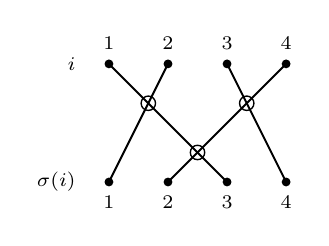
\begin{tikzpicture}[x=0.75cm, y=1.5cm, font=\scriptsize]
\foreach \i/\s in {1/3,2/1,3/4,4/2} {\draw[line width=0.7pt] (\i,1) -- (\s,0);}
\foreach \i in {1,2,3,4} {\fill (\i,1) circle (1.6pt); \node[above] at (\i,1.04) {$\i$}; \fill (\i,0) circle (1.6pt); \node[below] at (\i,-0.04) {$\i$};}
\foreach \x/\y in {1.6667/0.6667,2.5/0.25,3.3333/0.6667} {\draw[line width=0.5pt] (\x,\y) circle (2.6pt);}
\node[left] at (0.6,1) {$i$}; \node[left] at (0.6,0) {$\sigma(i)$};
\end{tikzpicture}}\hfill
\sdpanel{B}{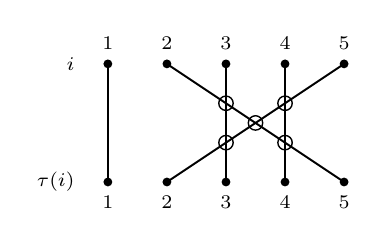
\begin{tikzpicture}[x=0.75cm, y=1.5cm, font=\scriptsize]
\foreach \i/\s in {1/1,2/5,3/3,4/4,5/2} {\draw[line width=0.7pt] (\i,1) -- (\s,0);}
\foreach \i in {1,2,3,4,5} {\fill (\i,1) circle (1.6pt); \node[above] at (\i,1.04) {$\i$}; \fill (\i,0) circle (1.6pt); \node[below] at (\i,-0.04) {$\i$};}
\foreach \x/\y in {3/0.6667,4/0.3333,3.5/0.5,3/0.3333,4/0.6667} {\draw[line width=0.5pt] (\x,\y) circle (2.6pt);}
\node[left] at (0.6,1) {$i$}; \node[left] at (0.6,0) {$\tau(i)$};
\end{tikzpicture}}
\caption{Inversions as crossings. Each $i$ in the upper row is joined to its image in the lower row, and every crossing (circled) is an inversion. (A) The permutation $\sigma=3142$ has three crossings and is odd. (B) The transposition $\tau=(2\,5)$ in $S_5$, which is $15342$ in one-line notation, has $2(5-2)-1=5$ crossings: the two long segments cross each other and each of the two vertical segments between them. Every transposition is odd.}
\label{fig:permutation-crossings}
\end{figure}

The count of inversions is defined through the order of the numbers $1,\ldots,n$, whereas a product of permutations only involves composition. The link between the two is the following product formula.

\begin{lemma}[Product formula for the sign]
\label{lem:sign-product}
For every $\sigma\in S_n$,
\[
\operatorname{sgn}\sigma=\prod_{1\le i<j\le n}\frac{\sigma(j)-\sigma(i)}{j-i} .
\]
More generally, the product does not change if each unordered pair $\{i,j\}$ contributes the factor $(\sigma(j)-\sigma(i))/(j-i)$ with its two elements taken in either order.
\end{lemma}

\begin{proof}
The factor for the pair $\{i,j\}$ is unchanged when $i$ and $j$ are exchanged, since numerator and denominator both change sign; this proves the last statement. The factor is negative exactly when $(i,j)$ is an inversion, so the sign of the product is $(-1)^{\operatorname{inv}(\sigma)}$. Its absolute value is $1$: as $\{i,j\}$ runs through all unordered pairs of distinct elements, so does $\{\sigma(i),\sigma(j)\}$, because $\sigma$ is a bijection; hence the numerators are, up to sign, the differences $|k-l|$ of all pairs $\{k,l\}$, which are also the denominators.
\end{proof}

\begin{theorem}[The sign is multiplicative]
\label{thm:sign-multiplicative}
For all $\sigma,\tau\in S_n$:
\begin{enumerate}
\item $\operatorname{sgn}(\sigma\tau)=\operatorname{sgn}\sigma\,\operatorname{sgn}\tau$, $\operatorname{sgn}\operatorname{id}=1$ and $\operatorname{sgn}\sigma^{-1}=\operatorname{sgn}\sigma$;
\item every transposition is odd, and a cycle of length $k$ has the sign $(-1)^{k-1}$;
\item if $\sigma$ is a product of $m$ transpositions, then $\operatorname{sgn}\sigma=(-1)^m$; in particular, the parity of the number of transpositions in such a product depends only on $\sigma$, and $\operatorname{sgn}\sigma=(-1)^{n-c(\sigma)}$.
\end{enumerate}
\end{theorem}

\begin{proof}
(i) By \cref{lem:sign-product},
\[
\operatorname{sgn}(\sigma\tau)=\prod_{i<j}\frac{\sigma(\tau(j))-\sigma(\tau(i))}{j-i}=\prod_{i<j}\frac{\sigma(\tau(j))-\sigma(\tau(i))}{\tau(j)-\tau(i)}\cdot\prod_{i<j}\frac{\tau(j)-\tau(i)}{j-i}.
\]
The second product is $\operatorname{sgn}\tau$. In the first, as $\{i,j\}$ runs through all pairs, so does $\{k,l\}=\{\tau(i),\tau(j)\}$, and the factor is $(\sigma(l)-\sigma(k))/(l-k)$ with the elements of the pair in some order; by the last statement of the lemma, the first product is $\operatorname{sgn}\sigma$. The identity has no inversions, and $1=\operatorname{sgn}(\sigma\sigma^{-1})=\operatorname{sgn}\sigma\operatorname{sgn}\sigma^{-1}$ gives $\operatorname{sgn}\sigma^{-1}=\operatorname{sgn}\sigma$, since both are $\pm1$.

(ii) Let $\tau=(a\,b)$ with $a<b$. In one-line notation, $\tau$ is the identity with the entries $a$ and $b$ exchanged. Its inversions are the pair $(a,b)$, the pairs $(a,k)$ with $a<k<b$, whose entries are $b>k$, and the pairs $(k,b)$ with $a<k<b$, whose entries are $k>a$; all other pairs keep their order. There are $1+2(b-a-1)$ inversions, an odd number. By \cref{prop:cycles}\,(ii) and (i) of this theorem, a cycle of length $k$ has the sign $(-1)^{k-1}$.

(iii) By (i) and (ii), a product of $m$ transpositions has the sign $(-1)^m$. If $\sigma$ is also a product of $m'$ transpositions, then $(-1)^m=(-1)^{m'}$, so $m$ and $m'$ have the same parity. The last formula follows from \cref{prop:cycles}\,(iii).
\end{proof}

Part (iii) shows that the sign could have been defined by counting transpositions, but then one would have to prove that the count has a well-defined parity, and the inversions are what makes this proof possible. For $\sigma=3142=(1\,3\,4\,2)$, the formula $(-1)^{n-c(\sigma)}=(-1)^{4-1}=-1$ agrees with the three inversions found above.

\begin{corollary}[Even and odd permutations]
\label{cor:even-odd}
For $n\ge2$, exactly half of the $n!$ permutations in $S_n$ are even. The map $\sigma\mapsto\sigma\tau$, for a fixed transposition $\tau$, is a bijection from the even permutations onto the odd ones.
\end{corollary}

\begin{proof}
The map $\sigma\mapsto\sigma\tau$ is a bijection of $S_n$, with the inverse $\rho\mapsto\rho\tau$, since $\tau\tau=\operatorname{id}$. By \cref{thm:sign-multiplicative}, $\operatorname{sgn}(\sigma\tau)=-\operatorname{sgn}\sigma$, so it maps the even permutations into the odd ones and the odd ones into the even ones. Hence the two sets have the same number of elements, $n!/2$.
\end{proof}

\subsection{Computing the Sign}

The definition suggests counting inversions, which takes about $n^2/2$ comparisons, and a variant of merge sort counts them with $O(n\log n)$ comparisons (Volume~IV). The formula $(-1)^{n-c(\sigma)}$ is cheaper still: one walks along the cycles, marking the elements visited, as in \cref{alg:permutation-sign}. Every element is visited once, so the cost is proportional to $n$. Elimination with row exchanges needs exactly this computation, since \cref{sec:det-elimination} shows that the sign of the permutation of $PA=LU$ enters the determinant; there, however, the sign is known for free, because the permutation is built from a counted number of exchanges.

\begin{algorithm}
\begin{algorithmic}[1]
\Require a permutation $\sigma$ of $\{1,\ldots,n\}$, given by the list $\sigma(1),\ldots,\sigma(n)$
\Ensure $\operatorname{sgn}\sigma$
\Name{PermutationSign}{\sigma}
\State $s\gets1$; mark all of $1,\ldots,n$ as unvisited
\For{$i=1,\ldots,n$}
  \If{$i$ is unvisited} \Comment{a new cycle starts at $i$}
    \State $j\gets i$; $k\gets0$
    \While{$j$ is unvisited}
      \State mark $j$ as visited; $j\gets\sigma(j)$; $k\gets k+1$
    \EndWhile
    \If{$k$ is even} \Comment{a cycle of length $k$ has the sign $(-1)^{k-1}$}
      \State $s\gets-s$
    \EndIf
  \EndIf
\EndFor
\State \Return $s$
\end{algorithmic}
\caption{The sign of a permutation by its cycles (\cref{thm:sign-multiplicative}\,(ii) and (iii)). Each element is visited once, so the work is proportional to $n$, and $n$ marks are stored.}
\label{alg:permutation-sign}
\end{algorithm}

\section{The Determinant}
\label{sec:det-definition}

\subsection{Multilinear Alternating Functions}

We regard a function of $n\times n$ matrices as a function of their $n$ columns and write $D(A)=D(\mathbf a_1,\ldots,\mathbf a_n)$ when $A$ has the columns $\mathbf a_1,\ldots,\mathbf a_n$.

\begin{definition}[Multilinear and alternating functions]
\label{def:multilinear-alternating}
Let $D\colon\mathbb F^{n\times n}\to\mathbb F$.
\begin{enumerate}
\item $D$ is \term{multilinear} (in the columns) if it is linear in each column when the other columns are held fixed: for every $j$, all columns $\mathbf a_i$ with $i\ne j$, all $\mathbf b,\mathbf c\in\mathbb F^n$ and all $s,t\in\mathbb F$,
\[
D(\mathbf a_1,\ldots,s\mathbf b+t\mathbf c,\ldots,\mathbf a_n)=s\,D(\mathbf a_1,\ldots,\mathbf b,\ldots,\mathbf a_n)+t\,D(\mathbf a_1,\ldots,\mathbf c,\ldots,\mathbf a_n),
\]
where $\mathbf b$, $\mathbf c$ and $s\mathbf b+t\mathbf c$ stand in position $j$.
\item $D$ is \term{alternating} if $D(A)=0$ whenever two columns of $A$ are equal.
\end{enumerate}
\end{definition}

The signed area $\mathcal A$ of \cref{sec:det-geometry} is a multilinear alternating function on $\mathbb R^{2\times2}$, and the triple product $\langle\mathbf a_1\times\mathbf a_2,\mathbf a_3\rangle$ is one on $\mathbb R^{3\times3}$. Multiples of a multilinear alternating function, and sums of two such functions, are again multilinear and alternating. Multilinearity does not mean linearity: by linearity in each of the $n$ columns, $D(tA)=t^nD(A)$, not $tD(A)$.

\begin{lemma}[Consequences of alternation]
\label{lem:alternating}
Let $D$ be multilinear and alternating, and $A\in\mathbb F^{n\times n}$.
\begin{enumerate}
\item Exchanging two columns of $A$ changes the sign of $D(A)$.
\item Adding a multiple of one column of $A$ to another column does not change $D(A)$.
\item If the columns of $A$ are linearly dependent, then $D(A)=0$.
\item For every $\tau\in S_n$, $D(\mathbf a_{\tau(1)},\ldots,\mathbf a_{\tau(n)})=\operatorname{sgn}\tau\;D(\mathbf a_1,\ldots,\mathbf a_n)$.
\end{enumerate}
\end{lemma}

\begin{proof}
(i) Fix all columns except those in the positions $k<l$, and let $f(\mathbf x,\mathbf y)$ be the value of $D$ with $\mathbf x$ in position $k$ and $\mathbf y$ in position $l$. By alternation and multilinearity,
\[
0=f(\mathbf x+\mathbf y,\mathbf x+\mathbf y)=f(\mathbf x,\mathbf x)+f(\mathbf x,\mathbf y)+f(\mathbf y,\mathbf x)+f(\mathbf y,\mathbf y)=f(\mathbf x,\mathbf y)+f(\mathbf y,\mathbf x).
\]
(ii) With the same notation, $f(\mathbf x+t\mathbf y,\mathbf y)=f(\mathbf x,\mathbf y)+t\,f(\mathbf y,\mathbf y)=f(\mathbf x,\mathbf y)$, and similarly in the other position. (iii) If the columns are dependent, one of them is a combination of the others, say $\mathbf a_k=\sum_{j\ne k}t_j\mathbf a_j$. By linearity in position $k$, $D(A)=\sum_{j\ne k}t_jD(A_j)$, where $A_j$ is $A$ with its $k$th column replaced by $\mathbf a_j$. Each $A_j$ has two equal columns, so $D(A_j)=0$. (iv) By \cref{prop:cycles}\,(iii), $\tau$ is a product $\rho_1\cdots\rho_m$ of transpositions, and we use induction on $m$; for $m=0$ there is nothing to prove. Let $m\ge1$, $\tau'\coloneqq\rho_1\cdots\rho_{m-1}$ and $\rho\coloneqq\rho_m=(k\,l)$, so that $\tau=\tau'\rho$. The matrix with the columns $\mathbf a_{\tau(j)}=\mathbf a_{\tau'(\rho(j))}$ is the matrix with the columns $\mathbf a_{\tau'(j)}$ with its columns $k$ and $l$ exchanged. By (i) and the induction hypothesis, its value is $-(-1)^{m-1}D(A)=(-1)^mD(A)$, which is $\operatorname{sgn}\tau\,D(A)$ by \cref{thm:sign-multiplicative}\,(iii).
\end{proof}

Property (i) says that an alternating function is \term{antisymmetric}. Over $\mathbb R$ and $\mathbb C$ the converse holds as well: if exchanging two equal columns changes the sign of $D(A)$, then $D(A)=-D(A)$, so $D(A)=0$. The step from $2D(A)=0$ to $D(A)=0$ is division by $2$, and the note below explains why the definition is nevertheless phrased with equal columns.

\begin{note}{Alternating and antisymmetric functions over other fields}
The algebraic part of this chapter uses only the rules of arithmetic in a field, and it holds for every field, for instance for the integers modulo a prime $p$ (\cref{sec:congruences}), over which exact computations with integer matrices are often carried out. In the field $\mathbb Z/2\mathbb Z$, however, $1+1=0$, so $-1=1$, and antisymmetry says nothing: every symmetric function is antisymmetric. The bilinear function $D(\mathbf u,\mathbf v)=u_1v_1$ on $(\mathbb Z/2\mathbb Z)^{2\times2}$ is antisymmetric there, but $D(\mathbf e_1,\mathbf e_1)=1\ne0$, and the uniqueness theorem below fails for it. Defining the determinant by alternation, as we do, keeps the algebraic results of the chapter true over every field; the results on volume, orientation and inequalities need the real numbers. Hoffman and Kunze develop the theory in this generality, over commutative rings~\cite[Chap.~5]{hoffman1971}.
\end{note}

\subsection{Uniqueness}

The computation that determined the signed area in \cref{sec:det-geometry} works in every dimension.

\begin{theorem}[Uniqueness of multilinear alternating functions]
\label{thm:det-uniqueness}
Let $D\colon\mathbb F^{n\times n}\to\mathbb F$ be multilinear and alternating. Then for every $A=(a_{ij})\in\mathbb F^{n\times n}$
\[
D(A)=D(I)\sum_{\sigma\in S_n}\operatorname{sgn}\sigma\;a_{\sigma(1)1}a_{\sigma(2)2}\cdots a_{\sigma(n)n} .
\]
\end{theorem}

\begin{proof}
The $j$th column of $A$ is $\mathbf a_j=\sum_{i=1}^na_{ij}\mathbf e_i$. Expanding by linearity in the first column, then in the second, and so on,
\[
D(A)=\sum_{i_1=1}^n\sum_{i_2=1}^n\cdots\sum_{i_n=1}^na_{i_11}a_{i_22}\cdots a_{i_nn}\,D(\mathbf e_{i_1},\mathbf e_{i_2},\ldots,\mathbf e_{i_n}).
\]
There is one term for each function $f\colon\{1,\ldots,n\}\to\{1,\ldots,n\}$, $j\mapsto i_j$, so $n^n$ terms in all. If $f$ is not injective, two of the vectors $\mathbf e_{i_j}$ are equal, and the term vanishes because $D$ is alternating. The injective functions from $\{1,\ldots,n\}$ to itself are the permutations (\cref{cor:finite}). For a permutation $\sigma$, \cref{lem:alternating}\,(iv) applied to the identity matrix with $\tau=\sigma$ gives $D(\mathbf e_{\sigma(1)},\ldots,\mathbf e_{\sigma(n)})=\operatorname{sgn}\sigma\,D(\mathbf e_1,\ldots,\mathbf e_n)=\operatorname{sgn}\sigma\,D(I)$. Only the $n!$ terms belonging to permutations remain, and they are the terms of the stated sum.
\end{proof}

The theorem says that a multilinear alternating function is determined by a single number, its value at the identity. It does not yet say that a nonzero such function exists: a priori the alternating property might force $D(I)=0$. We now show that the sum in the theorem is itself multilinear and alternating, with the value $1$ at the identity.

\subsection{Existence and the Definition}

\begin{theorem}[Existence of the determinant]
\label{thm:det-existence}
The function $\det\colon\mathbb F^{n\times n}\to\mathbb F$,
\begin{equation}
\det A\coloneqq\sum_{\sigma\in S_n}\operatorname{sgn}\sigma\prod_{j=1}^na_{\sigma(j)j},
\label{eq:leibniz}
\end{equation}
is multilinear and alternating, and $\det I=1$.
\end{theorem}

\begin{proof}
\emph{Multilinear.} Each term of \eqref{eq:leibniz} contains exactly one entry of the $j$th column, $a_{\sigma(j)j}$, as a factor. With the other columns fixed, each term is therefore a fixed number times one component of the $j$th column, a linear function of that column, and a sum of linear functions is linear.

\emph{Alternating.} Suppose that the columns $k<l$ of $A$ are equal, $a_{ik}=a_{il}$ for all $i$, and let $\tau\coloneqq(k\,l)$. By \cref{cor:even-odd}, $\sigma\mapsto\sigma\tau$ is a bijection from the even permutations onto the odd ones, so the terms of \eqref{eq:leibniz} come in pairs, one for an even $\sigma$ and one for $\sigma\tau$. In the product for $\sigma\tau$, the factor for $j\notin\{k,l\}$ is $a_{\sigma(j)j}$, the factor for $j=k$ is $a_{\sigma(l)k}=a_{\sigma(l)l}$, and the factor for $j=l$ is $a_{\sigma(k)l}=a_{\sigma(k)k}$. So the products for $\sigma$ and for $\sigma\tau$ are equal, while their signs are opposite, and each pair contributes $0$.

\emph{Normalisation.} For $A=I$ the product $\prod_j\delta_{\sigma(j)j}$ is $1$ if $\sigma(j)=j$ for every $j$ and $0$ otherwise. Only the identity contributes, with the sign $1$.
\end{proof}

\begin{definition}[Determinant]
\label{def:determinant}
The number $\det A$ of \eqref{eq:leibniz} is the \term{determinant} of $A\in\mathbb F^{n\times n}$. For the matrix with the columns $\mathbf a_1,\ldots,\mathbf a_n$ we also write $\det(\mathbf a_1,\ldots,\mathbf a_n)$, and the written-out matrix is sometimes enclosed in vertical bars,
\[
\det\begin{bmatrix}a_{11}&\cdots&a_{1n}\\\vdots&&\vdots\\a_{n1}&\cdots&a_{nn}\end{bmatrix}=\begin{vmatrix}a_{11}&\cdots&a_{1n}\\\vdots&&\vdots\\a_{n1}&\cdots&a_{nn}\end{vmatrix};
\]
we use the first form. Formula \eqref{eq:leibniz} is the \term{Leibniz formula}, or the expansion of the determinant over permutations.
\end{definition}

Taken together, the two theorems characterise the determinant.

\begin{corollary}[Characterisation of the determinant]
\label{cor:det-characterisation}
The determinant is the only multilinear alternating function on $\mathbb F^{n\times n}$ with the value $1$ at the identity. Every multilinear alternating function $D$ on $\mathbb F^{n\times n}$ satisfies $D(A)=D(I)\det A$.
\end{corollary}

\begin{proof}
By \cref{thm:det-existence}, $\det$ has the three properties, and by \cref{thm:det-uniqueness} every multilinear alternating $D$ equals $D(I)$ times the sum in \eqref{eq:leibniz}, which is $\det A$.
\end{proof}

The corollary is the tool of the next sections. To prove that some quantity equals $c\det A$, it suffices to show that the quantity is multilinear and alternating in the columns of $A$ and equals $c$ at the identity; no computation with the $n!$ terms is needed.

\subsection{Small Orders}

For $n=1$, $\det[a]=a$. For $n=2$, the permutations are $12$ (even) and $21$ (odd), and \eqref{eq:leibniz} gives $a_{11}a_{22}-a_{21}a_{12}$, the formula of \cref{prop:inverse-2x2}. For $n=3$ the six permutations are the even ones $123$, $231$, $312$, which are the identity and the two cycles of length $3$, and the odd ones $132$, $213$, $321$, which are the three transpositions. The Leibniz formula gives
\begin{equation}
\begin{aligned}
\det\begin{bmatrix}a_{11}&a_{12}&a_{13}\\a_{21}&a_{22}&a_{23}\\a_{31}&a_{32}&a_{33}\end{bmatrix}
&=a_{11}a_{22}a_{33}+a_{21}a_{32}a_{13}+a_{31}a_{12}a_{23}\\
&\quad-a_{11}a_{32}a_{23}-a_{21}a_{12}a_{33}-a_{31}a_{22}a_{13},
\end{aligned}
\label{eq:det3}
\end{equation}
and multiplying out the formula of \cref{sec:vectors-rn} produces the same six terms. So the definition agrees with the formulas used since \cref{ch:several-variables} for $n=2$ and $n=3$.

The six terms of \eqref{eq:det3} can be remembered by the \term{rule of Sarrus}: copy the first two columns to the right of the matrix; the three diagonals running down to the right carry the positive terms, and the three running up to the right the negative ones. The rule is particular to $n=3$. For $n=4$ the corresponding picture has eight diagonals, which produce only $8$ of the $4!=24$ terms of the determinant, and some of them with the wrong sign: the diagonal through $a_{12}$ running down to the right gives $a_{12}a_{23}a_{34}a_{41}$, whose permutation is a cycle of length $4$ and hence odd. The Leibniz formula itself is no better for computation: with $n!$ terms of $n$ factors each it needs about $n\cdot n!$ operations, and \cref{sec:det-elimination} replaces it by elimination.

For example,
\[
\det\begin{bmatrix}1&2&3\\4&5&6\\7&8&10\end{bmatrix}=50+96+84-48-80-105=-3,
\]
where the terms are listed in the order of \eqref{eq:det3}, whereas the matrix with the last entry $9$ instead of $10$ has the determinant $0$, in accordance with \cref{lem:alternating}\,(iii): its columns satisfy $\mathbf a_1-2\mathbf a_2+\mathbf a_3=\mathbf 0$.

\subsection{Triangular and Permutation Matrices}

For some matrices almost all terms of the Leibniz formula vanish.

\begin{proposition}[Triangular, diagonal and permutation matrices]
\label{prop:det-triangular}
\leavevmode
\begin{enumerate}
\item The determinant of an upper or a lower triangular matrix is the product of its diagonal entries; in particular $\det\operatorname{diag}(d_1,\ldots,d_n)=d_1\cdots d_n$.
\item For every $\sigma\in S_n$, the permutation matrix $P_\sigma$ of \cref{sec:special-matrices} has $\det P_\sigma=\operatorname{sgn}\sigma$.
\end{enumerate}
\end{proposition}

\begin{proof}
(i) Let $A$ be upper triangular, $a_{ij}=0$ for $i>j$. The product $\prod_ja_{\sigma(j)j}$ can be nonzero only if $\sigma(j)\le j$ for every $j$. Then $\sigma(1)=1$; and if $\sigma(i)=i$ for all $i<j$, then $\sigma(j)$, which is at most $j$ and differs from the values $1,\ldots,j-1$ already taken, equals $j$. So $\sigma=\operatorname{id}$, and $\det A=a_{11}a_{22}\cdots a_{nn}$. For lower triangular matrices the condition is $\sigma(j)\ge j$ for every $j$, and the same argument runs from $j=n$ downwards. (ii) $P_\sigma$ has the columns $\mathbf e_{\sigma(1)},\ldots,\mathbf e_{\sigma(n)}$, so by \cref{lem:alternating}\,(iv) with $A=I$, $\det P_\sigma=\operatorname{sgn}\sigma\det I=\operatorname{sgn}\sigma$.
\end{proof}

A triangular matrix is therefore invertible exactly when its determinant is nonzero, by \cref{thm:triangular}\,(ii); \cref{thm:det-invertible} below extends this to all square matrices. Part (ii) gives a second way of computing a sign: the permutation matrix of $3142$ is reduced to $I$ by three exchanges of columns, so its determinant, and the sign of $3142$, is $(-1)^3=-1$.

\begin{note}{The permanent}
Dropping the signs from the Leibniz formula gives the \emph{permanent} $\operatorname{per}A\coloneqq\sum_{\sigma}\prod_ja_{\sigma(j)j}$. It is multilinear, but symmetric instead of alternating, and it counts combinatorial objects: if $A$ is the $0$--$1$ matrix of a bipartite graph, $\operatorname{per}A$ is the number of perfect matchings, the ways of pairing every row with a column through an entry $1$. The difference in the sign changes everything computationally. Adding a multiple of one row to another changes the permanent, so elimination does not apply, and no method is known that computes the permanent of a general $n\times n$ matrix in a number of operations bounded by a polynomial in $n$. Valiant proved that computing the permanent of $0$--$1$ matrices is $\#\mathrm P$-complete~\cite{valiant1979}: a polynomial-time algorithm for it would give polynomial-time algorithms for every problem in the class $\#\mathrm P$ of counting problems, among them counting the solutions of any problem in NP, and would therefore imply $\mathrm P=\mathrm{NP}$. Whether such an algorithm exists is open, but it is widely conjectured that none does. The determinant, by contrast, costs a few multiples of $n^3$ operations, as \cref{sec:det-elimination} shows.
\end{note}

\section{Properties of the Determinant}
\label{sec:det-properties}

\subsection{The Transpose}

The definition treats columns and rows differently: each term of \eqref{eq:leibniz} picks one entry from every column. It also picks one entry from every row, since $\sigma$ is a bijection, and this is the reason why rows and columns play the same role after all.

\begin{theorem}[Determinant of the transpose]
\label{thm:det-transpose}
For every $A\in\mathbb F^{n\times n}$, $\det A^{\mathsf T}=\det A$. Consequently
\[
\det A=\sum_{\sigma\in S_n}\operatorname{sgn}\sigma\;a_{1\sigma(1)}a_{2\sigma(2)}\cdots a_{n\sigma(n)},
\]
and the determinant is multilinear and alternating in the rows of $A$ as well.
\end{theorem}

\begin{proof}
The $(i,j)$ entry of $A^{\mathsf T}$ is $a_{ji}$, so by definition $\det A^{\mathsf T}=\sum_\sigma\operatorname{sgn}\sigma\prod_ja_{j\sigma(j)}$. In the product $\prod_ja_{j\sigma(j)}$ we rename the index: as $j$ runs through $1,\ldots,n$, so does $i=\sigma(j)$, and $j=\sigma^{-1}(i)$; hence $\prod_ja_{j\sigma(j)}=\prod_ia_{\sigma^{-1}(i)i}$, since the factors of a product of numbers may be taken in any order. With $\rho\coloneqq\sigma^{-1}$ and $\operatorname{sgn}\rho=\operatorname{sgn}\sigma$ (\cref{thm:sign-multiplicative}\,(i)),
\[
\det A^{\mathsf T}=\sum_{\sigma\in S_n}\operatorname{sgn}\sigma^{-1}\prod_ia_{\sigma^{-1}(i)i}=\sum_{\rho\in S_n}\operatorname{sgn}\rho\prod_ia_{\rho(i)i}=\det A,
\]
because $\sigma\mapsto\sigma^{-1}$ is a bijection of $S_n$. The displayed formula is the definition applied to $A^{\mathsf T}$. The rows of $A$ are the columns of $A^{\mathsf T}$, so the determinant, as a function of the rows, is the multilinear alternating function $A\mapsto\det A^{\mathsf T}$.
\end{proof}

The displayed formula is the one used in the proof of \cref{thm:invertible-matrices}; the theorem shows that it defines the same determinant. Every statement about columns now has a counterpart for rows: by \cref{lem:alternating}, exchanging two rows changes the sign, adding a multiple of one row to another changes nothing, and a matrix with linearly dependent rows has the determinant $0$.

\subsection{Row Operations and Elementary Matrices}

The three row operations of \cref{def:row-operations} affect the determinant in a simple way, and so do the corresponding column operations.

\begin{proposition}[Determinants and elementary operations]
\label{prop:det-elementary}
Let $A\in\mathbb F^{n\times n}$, $i\ne j$ and $c\in\mathbb F$.
\begin{enumerate}
\item Exchanging two rows, or two columns, of $A$ multiplies $\det A$ by $-1$.
\item Multiplying a row, or a column, of $A$ by $c$ multiplies $\det A$ by $c$.
\item Adding $c$ times one row to another row, or $c$ times one column to another column, does not change $\det A$.
\end{enumerate}
For the elementary matrices of \cref{sec:elimination}, $\det P_{ij}=-1$, $\det D_i(c)=c$ and $\det E_{ij}(c)=1$, and for each of them $\det(EA)=\det E\det A=\det(AE)$.
\end{proposition}

\begin{proof}
For columns, (i) and (iii) are \cref{lem:alternating}\,(i) and (ii), and (ii) is linearity in one column. For rows they follow by \cref{thm:det-transpose}, since a row operation on $A$ is a column operation on $A^{\mathsf T}$. The values $\det P_{ij}$, $\det D_i(c)$ and $\det E_{ij}(c)$ are obtained by applying the operations to $I$, which has $\det I=1$; the last value also follows from \cref{prop:det-triangular}, since $E_{ij}(c)$ is triangular with the diagonal entries $1$. Finally, $EA$ is $A$ with the row operation of $E$ applied, and $AE$ is $A$ with the corresponding column operation applied (\cref{prop:elementary-matrices}), so both determinants equal $\det E\det A$ by (i) to (iii).
\end{proof}

The proposition gives the most practical way of computing determinants by hand: reduce the matrix to triangular form by row operations, keeping track of exchanges and scalings. For the matrix of the example above, subtracting $4$ and $7$ times the first row from the others, and then twice the new second row from the third, changes nothing:
\[
\det\begin{bmatrix}1&2&3\\4&5&6\\7&8&10\end{bmatrix}=\det\begin{bmatrix}1&2&3\\0&-3&-6\\0&-6&-11\end{bmatrix}=\det\begin{bmatrix}1&2&3\\0&-3&-6\\0&0&1\end{bmatrix}=1\cdot(-3)\cdot1=-3 .
\]
\Cref{sec:det-elimination} turns this procedure into an algorithm.

\subsection{Invertibility}

\begin{theorem}[The determinant criterion]
\label{thm:det-invertible}
A matrix $A\in\mathbb F^{n\times n}$ is invertible if and only if $\det A\ne0$. Thus the condition
\begin{enumerate}
\item[(x)] $\det A\ne0$
\end{enumerate}
can be added to the equivalent conditions of \cref{thm:invertible}.
\end{theorem}

\begin{proof}
If $A$ is singular, there is $\mathbf x\ne\mathbf 0$ with $A\mathbf x=\mathbf 0$ (\cref{thm:invertible}), that is, $\sum_jx_j\mathbf a_j=\mathbf 0$, so the columns of $A$ are linearly dependent and $\det A=0$ by \cref{lem:alternating}\,(iii). If $A$ is invertible, it is a product $E_1E_2\cdots E_k$ of elementary matrices (\cref{thm:invertible}), and by \cref{prop:det-elementary}, applied $k$ times,
\[
\det A=\det E_1\det(E_2\cdots E_k)=\cdots=\det E_1\det E_2\cdots\det E_k\det I ,
\]
a product of the nonzero numbers $-1$, $c\ne0$ and $1$.
\end{proof}

\Cref{thm:invertible} and its proof hold for complex matrices, as \cref{ch:linear-systems} observed, and so does this theorem. It completes part (i) of \cref{thm:invertible-matrices}, whose remaining equivalences \cref{thm:invertible} proved. In geometric terms, the columns of a singular matrix lie in a hyperplane (\cref{prop:singular-image}), and the parallelepiped they span is flat; its signed volume is $0$.

\subsection{The Product Rule}

\begin{theorem}[Product rule]
\label{thm:det-product}
For all $A,B\in\mathbb F^{n\times n}$, $\det(AB)=\det A\det B$.
\end{theorem}

\begin{proof}
Fix $A$, and let $D(B)\coloneqq\det(AB)$. The $j$th column of $AB$ is $A\mathbf b_j$ (\cref{thm:four-readings}), and $\mathbf b\mapsto A\mathbf b$ is linear, so $D$ is multilinear in the columns of $B$. If two columns of $B$ are equal, the same two columns of $AB$ are equal, and $D(B)=0$. Finally $D(I)=\det A$. By \cref{cor:det-characterisation}, $D(B)=D(I)\det B=\det A\det B$.
\end{proof}

The proof uses no formula and no elimination, only the uniqueness of the determinant: the function $B\mapsto\det(AB)$ is multilinear and alternating, so it can only be a multiple of $\det B$, and the multiple is found at $B=I$. Geometrically, $AB$ maps the unit cube first by $B$, multiplying volumes by $|\det B|$, and then by $A$, multiplying them by $|\det A|$; \cref{sec:det-volume} makes this precise.

\begin{corollary}[Consequences of the product rule]
\label{cor:det-product}
Let $A,B\in\mathbb F^{n\times n}$ and $c\in\mathbb F$.
\begin{enumerate}
\item If $A$ is invertible, $\det A^{-1}=1/\det A$.
\item $\det A^k=(\det A)^k$ for $k\in\mathbb N$, and for all integers $k$ if $A$ is invertible.
\item $\det(cA)=c^n\det A$.
\item $\det(AB)=\det(BA)$, although $AB\ne BA$ in general.
\item If $P$ is invertible, $\det(P^{-1}AP)=\det A$: similar matrices have the same determinant.
\item $AB$ is invertible if and only if both $A$ and $B$ are.
\end{enumerate}
\end{corollary}

\begin{proof}
(i) $\det A\det A^{-1}=\det(AA^{-1})=\det I=1$. (ii) By induction on $k$, and for negative $k$ by (i). (iii) $cA=(cI)A$, and $\det(cI)=c^n$ by \cref{prop:det-triangular}. (iv) Both sides equal $\det A\det B$. (v) $\det P^{-1}\det A\det P=\det A$ by (i). (vi) $\det(AB)\ne0$ if and only if $\det A\ne0$ and $\det B\ne0$; apply \cref{thm:det-invertible}.
\end{proof}

The determinant respects products but not sums. In general $\det(A+B)\ne\det A+\det B$: for $n\ge2$, $\det(I+I)=2^n$, while $\det I+\det I=2$; \cref{ch:linear-maps} used the case $\det(2I)=4\ne2\det I$ to show that the determinant of $2\times2$ matrices is not linear. Nor is there any useful formula for $\det(A+B)$ in terms of $\det A$ and $\det B$: the matrices $\operatorname{diag}(1,0)$ and $\operatorname{diag}(0,1)$ both have the determinant $0$, while their sum $I$ has the determinant $1$, and their difference the determinant $-1$. \Cref{sec:det-block} shows what can be said when $B$ has rank one.

\subsection{The Determinant of an Operator}

Part (v) of the corollary adds the determinant to the similarity invariants of \cref{prop:similarity-invariants}, and it makes the following definition possible.

\begin{proposition}[Determinant of an operator]
\label{prop:det-operator}
Let $V$ be a vector space of dimension $n\ge1$ and $T$ an operator on $V$. The number $\det T\coloneqq\det[T]_{\mathcal B}$ does not depend on the basis $\mathcal B$ of $V$. Moreover $\det(ST)=\det S\det T$ for operators $S$ and $T$ on $V$, $\det\operatorname{id}_V=1$, and $T$ is invertible if and only if $\det T\ne0$.
\end{proposition}

\begin{proof}
For two bases $\mathcal B$ and $\mathcal B'$, $[T]_{\mathcal B'}=P^{-1}[T]_{\mathcal B}P$ with an invertible $P$ (\cref{sec:similarity}), and the two matrices have the same determinant by \cref{cor:det-product}\,(v). By \cref{thm:composition-matrix}, $[ST]_{\mathcal B}=[S]_{\mathcal B}[T]_{\mathcal B}$ and $[\operatorname{id}]_{\mathcal B}=I$, so the product rule gives the second statement, and $T$ is invertible if and only if $[T]_{\mathcal B}$ is, which by \cref{thm:det-invertible} means $\det[T]_{\mathcal B}\ne0$.
\end{proof}

The determinant of an operator can be computed in whichever basis is most convenient. Differentiation on $\mathcal P_n$, $n\ge1$, has a strictly upper triangular matrix in the monomial basis, so its determinant is $0$, as it must be for an operator with the nonzero kernel of constants. The shift $p(x)\mapsto p(x+1)$ on $\mathcal P_n$ maps $x^k$ to $x^k$ plus terms of lower degree, by the binomial theorem, so its matrix is unit upper triangular and its determinant is $1$. The substitution $p(x)\mapsto p(2x)$ maps $x^k$ to $2^kx^k$ and has the determinant $1\cdot2\cdot4\cdots2^n=2^{n(n+1)/2}$. The transposition $X\mapsto X^{\mathsf T}$ on $\mathbb F^{n\times n}$ permutes the basis of matrix units: it fixes the $n$ units $E_{ii}$ and exchanges $E_{ij}$ and $E_{ji}$ for each of the $n(n-1)/2$ pairs $i<j$. Its matrix is the permutation matrix of a product of $n(n-1)/2$ disjoint transpositions, and its determinant is $(-1)^{n(n-1)/2}$ by \cref{prop:det-triangular}\,(ii) and \cref{thm:sign-multiplicative}; for $n=2$ it is $-1$, and for $n=4$ it is $1$.

For a linear map $T\colon V\to W$ between two different spaces of the same dimension, there is no determinant. Changing the bases replaces the matrix by $Q^{-1}[T]P$ (\cref{thm:change-of-basis-map}), whose determinant is $\det[T]\det P/\det Q$, and since $P$ and $Q$ can be chosen independently, this number can be made any nonzero multiple of $\det[T]$. Only whether it is zero has a meaning independent of the bases: by \cref{thm:composition-matrix}, it is zero exactly when $T$ is not an isomorphism.

\subsection{Conjugates, Orthogonal and Unitary Matrices}

\begin{proposition}[Determinants of conjugates, orthogonal and unitary matrices]
\label{prop:det-unitary}
\leavevmode
\begin{enumerate}
\item For $A\in\mathbb C^{n\times n}$, $\det\bar A=\overline{\det A}$ and $\det A^{\mathsf H}=\overline{\det A}$. The determinant of a real matrix is real.
\item If $Q\in\mathbb R^{n\times n}$ is orthogonal, then $\det Q=\pm1$.
\item If $U\in\mathbb C^{n\times n}$ is unitary, then $|\det U|=1$.
\end{enumerate}
\end{proposition}

\begin{proof}
(i) Conjugation respects sums and products of complex numbers (\cref{prop:conjugate}), and the signs are real; applying it to \eqref{eq:leibniz} gives $\overline{\det A}=\det\bar A$, and $\det A^{\mathsf H}=\det\bar A^{\mathsf T}=\det\bar A$ by \cref{thm:det-transpose}. The Leibniz formula involves only sums and products of the entries. (ii) $1=\det(Q^{\mathsf T}Q)=\det Q^{\mathsf T}\det Q=(\det Q)^2$. (iii) $1=\det(U^{\mathsf H}U)=\overline{\det U}\det U=|\det U|^2$.
\end{proof}

The rotations $R_\varphi$ of \cref{sec:matrices-linear-maps} have the determinant $\cos^2\varphi+\sin^2\varphi=1$, and the reflections $S_\alpha$ the determinant $-\cos^22\alpha-\sin^22\alpha=-1$. By the description of the orthogonal $2\times2$ matrices after \cref{thm:orthogonal}, the orthogonal matrices with determinant $1$ in the plane are exactly the rotations, and those with determinant $-1$ exactly the reflections. In every dimension, orthogonal matrices with the determinant $1$ are called \term{rotations}, or proper orthogonal matrices, and they are the rigid motions that fix the origin and preserve orientation in the sense of \cref{sec:det-volume}. A permutation matrix is a rotation exactly when its permutation is even, and the Householder reflection of \cref{prop:householder} has the determinant $-1$ (\cref{sec:det-block}). The converse of (ii) fails: the shear $E_{12}(1)$ has the determinant $1$ but is not orthogonal, since it changes the length of $\mathbf e_2$.

\section{Computing Determinants by Elimination}
\label{sec:det-elimination}

\subsection{The Determinant from \texorpdfstring{$PA=LU$}{PA = LU}}

Gaussian elimination reduces a square matrix to triangular form by operations whose effect on the determinant is known, and the factorisation $PA=LU$ of \cref{thm:plu} records the result.

\begin{theorem}[Determinant by elimination]
\label{thm:det-plu}
Let $PA=LU$, where $A\in\mathbb F^{n\times n}$, $L$ is unit lower triangular, $U$ is upper triangular, and $P$ is a product of $s$ exchange matrices. Then
\[
\det A=(-1)^s\,u_{11}u_{22}\cdots u_{nn}.
\]
\end{theorem}

\begin{proof}
By the product rule, $\det P\det A=\det L\det U$. Here $\det L=1$ and $\det U=u_{11}\cdots u_{nn}$ by \cref{prop:det-triangular}, and $\det P=(-1)^s$ by \cref{prop:det-elementary} and the product rule. Since $(-1)^s(-1)^s=1$, multiplying by $(-1)^s$ gives the formula.
\end{proof}

The matrix $P$ is the permutation matrix $P_\pi$ of the permutation $\pi$ that the exchanges produce, so the sign can also be written as $\operatorname{sgn}\pi$ (\cref{prop:det-triangular}); different sequences of exchanges that produce the same $P$ have numbers $s$ of the same parity, by \cref{thm:sign-multiplicative}\,(iii). The theorem fulfils the promise made after \cref{thm:plu}: the determinant is, up to sign, the product of the pivots. For the matrix of the system \eqref{eq:example-system}, elimination without exchanges finds the pivots $2$, $1$ and $1$, so its determinant is $2$. With partial pivoting the work is different and the answer the same: the first column has its largest entry $-4$ in the second row, and after exchanging the first two rows and eliminating,
\[
\begin{bmatrix}-4&-1&3\\2&1&-1\\2&3&2\end{bmatrix}\longrightarrow\begin{bmatrix}-4&-1&3\\0&1/2&1/2\\0&5/2&7/2\end{bmatrix}\longrightarrow\begin{bmatrix}-4&-1&3\\0&5/2&7/2\\0&0&-1/5\end{bmatrix},
\]
where the second step exchanges the last two rows and subtracts $1/5$ times the new second row from the third. Two exchanges were made, and $\det A=(-1)^2\cdot(-4)\cdot(5/2)\cdot(-1/5)=2$. For the second difference matrix $T_n$ of \cref{sec:special-matrices}, elimination without exchanges produces the pivots $2,3/2,4/3,\ldots,(n+1)/n$, as \cref{sec:special-systems} found, and the product telescopes to $\det T_n=n+1$.

A hand computation of order $4$ shows the bookkeeping. For
\[
A=\begin{bmatrix}0&2&0&2\\1&-1&-2&-2\\-1&1&3&-2\\-1&-1&2&3\end{bmatrix},
\]
the first pivot position holds $0$, and we exchange the first two rows ($s=1$). Adding the new first row to the third and to the fourth row, and then the second row to the fourth, gives
\[
\begin{bmatrix}1&-1&-2&-2\\0&2&0&2\\-1&1&3&-2\\-1&-1&2&3\end{bmatrix}\longrightarrow\begin{bmatrix}1&-1&-2&-2\\0&2&0&2\\0&0&1&-4\\0&-2&0&1\end{bmatrix}\longrightarrow\begin{bmatrix}1&-1&-2&-2\\0&2&0&2\\0&0&1&-4\\0&0&0&3\end{bmatrix},
\]
which is upper triangular; the third column needs no elimination, since the entry below its pivot is already $0$. So $\det A=(-1)^1\cdot1\cdot2\cdot1\cdot3=-6$. In exact arithmetic any nonzero entry may serve as a pivot, and by hand one chooses whatever keeps the numbers simple; in floating-point arithmetic the choice matters for accuracy (\cref{sec:pivoting}).

\subsection{Pivots and Leading Principal Minors}

The determinant of a square submatrix of $A$, formed by some $k$ of its rows and some $k$ of its columns, is a \term{minor} of order $k$ of $A$. The \term{leading principal minors} $\Delta_k\coloneqq\det A_k$, $k=1,\ldots,n$, are those of the leading principal submatrices $A_k$ of \cref{thm:lu-existence}; they appeared in Sylvester's criterion of \cref{thm:definiteness-criteria}. They are the products of the pivots.

\begin{proposition}[Pivots and leading principal minors]
\label{prop:pivots-minors}
Let $A=LU$ with $L$ unit lower triangular and $U$ upper triangular. Then $\Delta_k=u_{11}u_{22}\cdots u_{kk}$ for $k=1,\ldots,n$, and if $\Delta_{k-1}\ne0$, the $k$th pivot is
\[
u_{kk}=\frac{\Delta_k}{\Delta_{k-1}}\qquad(\Delta_0\coloneqq1).
\]
An invertible matrix has an LU factorisation if and only if all its leading principal minors are nonzero. If $A$ is symmetric and $A=LDL^{\mathsf T}$ as in \cref{prop:ldu}, then $\Delta_k=d_1\cdots d_k$; in particular all pivots $d_k$ are positive if and only if all $\Delta_k$ are positive.
\end{proposition}

\begin{proof}
By the observation before \cref{thm:lu-existence}, $A_k=L_kU_k$, where $L_k$ is unit lower triangular and $U_k$ upper triangular with the diagonal entries $u_{11},\ldots,u_{kk}$; the product rule and \cref{prop:det-triangular} give $\Delta_k=u_{11}\cdots u_{kk}$, and dividing by $\Delta_{k-1}$ gives $u_{kk}$. The criterion for an LU factorisation is \cref{thm:lu-existence}, with the invertibility of each $A_k$ expressed by $\Delta_k\ne0$ (\cref{thm:det-invertible}). For symmetric $A=LDL^{\mathsf T}$ the pivots are $d_k=u_{kk}$, and if all $\Delta_k$ are positive, so are all $d_k=\Delta_k/\Delta_{k-1}$; conversely positive pivots give positive products.
\end{proof}

For $T_n$, the leading principal submatrices are $T_1,\ldots,T_n$ themselves, so $\Delta_k=k+1$ and $u_{kk}=(k+1)/k$, in agreement with the pivots above. The last statement of the proposition is the link between Sylvester's criterion and elimination that the proof of \cref{thm:definiteness-criteria} used; that positive pivots characterise positive definite matrices is proved in Chapter~20. Formulas such as $u_{kk}=\Delta_k/\Delta_{k-1}$ are useful in theory, and they are a poor way to compute: a pivot is obtained far more cheaply by elimination itself.

\subsection{The Algorithm and Its Cost}

\Cref{alg:det-lu} is the method by which determinants are computed in practice. It is \cref{alg:lu} with a running product of the pivots and a sign that changes with each exchange.

\begin{algorithm}
\begin{algorithmic}[1]
\Require $A=(a_{ij})\in\mathbb F^{n\times n}$
\Ensure $\det A$; $A$ is overwritten by the factors of $PA=LU$
\Name{Determinant}{A}
\State $d\gets1$
\For{$k=1,\ldots,n$}
  \State choose $r\ge k$ with $|a_{rk}|=\max_{i\ge k}|a_{ik}|$
  \If{$a_{rk}=0$} \Comment{the column is zero from row $k$ on: $A$ is singular}
    \State \Return $0$
  \EndIf
  \If{$r\ne k$}
    \State exchange the rows $k$ and $r$ of $A$; $d\gets-d$
  \EndIf
  \State $d\gets d\cdot a_{kk}$
  \For{$i=k+1,\ldots,n$}
    \State $a_{ik}\gets a_{ik}/a_{kk}$
    \For{$j=k+1,\ldots,n$}
      \State $a_{ij}\gets a_{ij}-a_{ik}a_{kj}$
    \EndFor
  \EndFor
\EndFor
\State \Return $d$
\end{algorithmic}
\caption{The determinant by Gaussian elimination with partial pivoting (\cref{thm:det-plu}). The work is that of \cref{alg:lu}, about $2n^3/3$ operations, plus one multiplication by each pivot.}
\label{alg:det-lu}
\end{algorithm}

If a column is zero from the diagonal down, the matrix is singular by the argument of \cref{prop:gauss-singular}, and the algorithm returns $0$ at once. By \cref{prop:elimination-cost} the elimination costs $2n^3/3-n^2/2-n/6$ operations, to which the product of the $n$ pivots adds $n-1$ multiplications. The Leibniz formula needs $n!$ products of $n$ factors, that is $n!(n-1)$ multiplications, and $n!-1$ additions, $n\cdot n!-1$ operations in all. \Cref{tab:det-cost} compares the two counts. Already for $n=10$ the formula needs some sixty thousand times as many operations, and for $n=20$ it needs about $4.9\times10^{19}$ operations, which at the highest rate measured in \cref{tab:solve-timing}, $8.3\times10^{11}$ operations per second, would take about two years. Elimination needs $5149$ operations for $n=20$.

\begin{table}
\sdfloat{%
\begin{sdtable}{colspec={rlll}, row{1}={font=\small\bfseries}}
\toprule
$n$ & terms $n!$ & Leibniz formula & elimination \\
\midrule
$2$ & $2$ & $3$ & $4$ \\
$5$ & $120$ & $599$ & $74$ \\
$10$ & $3\,628\,800$ & $3.6\times10^{7}$ & $624$ \\
$20$ & $2.4\times10^{18}$ & $4.9\times10^{19}$ & $5149$ \\
$50$ & $3.0\times10^{64}$ & $1.5\times10^{66}$ & $82\,124$ \\
\bottomrule
\end{sdtable}}{The number of arithmetic operations for the determinant of an $n\times n$ matrix by the Leibniz formula \eqref{eq:leibniz}, $n\cdot n!-1$, and by elimination, $2n^3/3-n^2/2-n/6+(n-1)$, rounded to two digits where they are large.\label{tab:det-cost}}
\end{table}

Elimination also produces the determinant exactly when it is carried out in exact arithmetic, for instance with rational numbers. For integer matrices the fractions can be avoided altogether, at the price of a division in every update that is known to be exact.

\begin{note}{Fraction-free elimination}
Elimination on an integer matrix in rational arithmetic creates fractions whose numerators and denominators may grow quickly, and reducing them by greatest common divisors is expensive. Bareiss~\cite{bareiss1968} observed that the update
\[
a_{ij}^{(k)}=\frac{a_{kk}^{(k-1)}a_{ij}^{(k-1)}-a_{ik}^{(k-1)}a_{kj}^{(k-1)}}{a_{k-1,k-1}^{(k-2)}}\qquad(i,j>k),
\]
with $a_{00}^{(-1)}\coloneqq1$ and $a_{ij}^{(0)}\coloneqq a_{ij}$, divides exactly: every intermediate entry $a_{ij}^{(k)}$ is the minor of $A$ formed by the rows $1,\ldots,k,i$ and the columns $1,\ldots,k,j$, an integer, and the last one, $a_{nn}^{(n-1)}$, is $\det A$ (if a pivot vanishes, rows are exchanged and the sign is recorded). Being minors, the intermediate integers are bounded by Hadamard's inequality (\cref{thm:hadamard}) applied to submatrices, so the length of the integers stays under control. Cohen describes the method among the algorithms of exact linear algebra over the integers~\cite{cohen1993}.
\end{note}

\begin{note}{The complexity of the determinant}
The count $2n^3/3$ is not the end of the story. Bunch and Hopcroft~\cite{bunch1974} showed that the LU factorisation, and with it the determinant, can be computed by recursive block elimination with $O(n^\alpha)$ operations whenever matrices can be multiplied with $O(n^\alpha)$ operations, so that the exponent $\omega$ of the note on Strassen's algorithm in \cref{sec:block-matrices} bounds the cost of determinants as well; with Strassen's algorithm~\cite{strassen1969}, $\alpha=\log_27\approx2.81$. The block step is the factorisation of \cref{thm:schur-complement}, with the determinant formula of \cref{thm:det-schur}. In practice determinants of dense matrices are computed by \cref{alg:det-lu} in its blocked form, as in the LAPACK library~\cite{golub2013}.
\end{note}

\section{Cofactor Expansion}
\label{sec:cofactor}

\subsection{Minors, Cofactors and the Expansion}

\Cref{ch:several-variables} computed $3\times3$ determinants by expanding along the first row into $2\times2$ determinants. The expansion works along every row and every column, and in every dimension.

\begin{definition}[Minors and cofactors]
\label{def:cofactor}
Let $A\in\mathbb F^{n\times n}$ with $n\ge2$. The \term{minor} $M_{ij}$ is the determinant of the $(n-1)\times(n-1)$ matrix obtained from $A$ by deleting the $i$th row and the $j$th column, and the \term{cofactor} of the entry $a_{ij}$ is $C_{ij}\coloneqq(-1)^{i+j}M_{ij}$.
\end{definition}

The signs $(-1)^{i+j}$ form a checkerboard pattern, beginning with $+$ in the upper left corner:
\[
\begin{bmatrix}+&-&+&\cdots\\-&+&-&\cdots\\+&-&+&\cdots\\\vdots&\vdots&\vdots&\ddots\end{bmatrix}.
\]

\begin{lemma}[A column of the identity]
\label{lem:unit-column}
If the $j$th column of $A\in\mathbb F^{n\times n}$ is $\mathbf e_i$, then $\det A=C_{ij}=(-1)^{i+j}M_{ij}$.
\end{lemma}

\begin{proof}
Move the $j$th column to the front by $j-1$ exchanges of neighbouring columns, which keeps the other columns in their order, and then the $i$th row to the top by $i-1$ exchanges of neighbouring rows. By \cref{prop:det-elementary} this multiplies the determinant by $(-1)^{i+j-2}=(-1)^{i+j}$, and it produces a matrix
\[
B=\begin{bmatrix}1&\mathbf r^{\mathsf T}\\\mathbf 0&A'\end{bmatrix},
\]
where $A'$ is $A$ with the $i$th row and the $j$th column deleted, so that $\det A'=M_{ij}$. In the Leibniz formula for $B$, the first column is $\mathbf e_1$, so only the permutations with $\sigma(1)=1$ contribute, with the factor $b_{11}=1$. Such a $\sigma$ permutes $\{2,\ldots,n\}$ and has no inversion involving the position $1$; renumbering $2,\ldots,n$ as $1,\ldots,n-1$, it becomes a permutation of $\{1,\ldots,n-1\}$ with the same inversions, and its term becomes the corresponding term of the Leibniz formula for $A'$. So $\det B=\det A'=M_{ij}$, and $\det A=(-1)^{i+j}M_{ij}$.
\end{proof}

\begin{theorem}[Laplace expansion]
\label{thm:laplace-expansion}
Let $A\in\mathbb F^{n\times n}$ with $n\ge2$. For every column $j$ and every row $i$,
\[
\det A=\sum_{k=1}^na_{kj}C_{kj}\qquad\text{and}\qquad\det A=\sum_{k=1}^na_{ik}C_{ik},
\]
the \term{expansions} of $\det A$ along the $j$th column and along the $i$th row.
\end{theorem}

\begin{proof}
The $j$th column is $\mathbf a_j=\sum_ka_{kj}\mathbf e_k$. By linearity in that column, $\det A=\sum_ka_{kj}\det A^{(k)}$, where $A^{(k)}$ is $A$ with its $j$th column replaced by $\mathbf e_k$. By \cref{lem:unit-column}, $\det A^{(k)}$ is $(-1)^{k+j}$ times the minor of $A^{(k)}$ obtained by deleting the $k$th row and the $j$th column; this deletes the replaced column, so the minor is $M_{kj}$, and $\det A^{(k)}=C_{kj}$. The expansion along a row is the expansion of $A^{\mathsf T}$ along a column, since $\det A^{\mathsf T}=\det A$ and the cofactors of $A^{\mathsf T}$ are those of $A$ with the indices exchanged.
\end{proof}

The expansion is most useful along a row or column with many zeros. For the matrix $A$ of order $4$ in \cref{sec:det-elimination}, the first row $(0,2,0,2)$ has two zeros, and
\[
\det A=-2M_{12}-2M_{14}=-2\det\begin{bmatrix}1&-2&-2\\-1&3&-2\\-1&2&3\end{bmatrix}-2\det\begin{bmatrix}1&-1&-2\\-1&1&3\\-1&-1&2\end{bmatrix}=-2\cdot1-2\cdot2=-6,
\]
in agreement with elimination; the two $3\times3$ determinants are $1$ and $2$ by \eqref{eq:det3}. For the Jacobian matrix of spherical coordinates in \cref{sec:inverse-implicit}, whose last row is $(\cos\theta,-r\sin\theta,0)$, the expansion along that row is
\[
\cos\theta\cdot\det\begin{bmatrix}r\cos\theta\cos\varphi&-r\sin\theta\sin\varphi\\r\cos\theta\sin\varphi&r\sin\theta\cos\varphi\end{bmatrix}+r\sin\theta\cdot\det\begin{bmatrix}\sin\theta\cos\varphi&-r\sin\theta\sin\varphi\\\sin\theta\sin\varphi&r\sin\theta\cos\varphi\end{bmatrix},
\]
where the sign of the second cofactor, $(-1)^{3+2}=-1$, has cancelled against the entry $-r\sin\theta$. The two $2\times2$ determinants are $r^2\sin\theta\cos\theta$ and $r\sin^2\theta$, so the determinant is $r^2\sin\theta\cos^2\theta+r^2\sin^3\theta=r^2\sin\theta$, the value used in \cref{sec:change-variables}; the theorem justifies the expansion along the last row that \cref{sec:inverse-implicit} anticipated.

As a method of computation for general matrices, the expansion is no better than the Leibniz formula: expanding recursively until the minors have order $1$ produces exactly the $n!$ terms of \eqref{eq:leibniz}. Its value lies in matrices with structure, in symbolic computations, and in the formulas that follow.

\subsection{The Adjugate and the Inverse}

Expanding with the cofactors of a different column gives zero.

\begin{proposition}[Expansion with alien cofactors]
\label{prop:alien-cofactors}
For $A\in\mathbb F^{n\times n}$, $n\ge2$, and columns $j\ne l$, $\sum_ka_{kl}C_{kj}=0$; for rows $i\ne l$, $\sum_ka_{lk}C_{ik}=0$.
\end{proposition}

\begin{proof}
Let $B$ be $A$ with its $j$th column replaced by its $l$th column. $B$ has two equal columns, so $\det B=0$. The cofactors $C_{kj}$ do not involve the $j$th column, so they are the same for $A$ and $B$, and the expansion of $\det B$ along its $j$th column is $\sum_ka_{kl}C_{kj}$. The statement for rows follows by transposition.
\end{proof}

\begin{definition}[Adjugate]
\label{def:adjugate}
The \term{adjugate} of $A\in\mathbb F^{n\times n}$, $n\ge2$, is the transpose of the matrix of cofactors: $\operatorname{adj}A\in\mathbb F^{n\times n}$ has the entries $(\operatorname{adj}A)_{ij}\coloneqq C_{ji}$. For $n=1$ we put $\operatorname{adj}A\coloneqq[1]$.
\end{definition}

\begin{theorem}[Adjugate formula]
\label{thm:adjugate}
For every $A\in\mathbb F^{n\times n}$,
\[
A\operatorname{adj}A=(\operatorname{adj}A)A=(\det A)I .
\]
Consequently, if $\det A\ne0$, then $A^{-1}=\operatorname{adj}A/\det A$: the entry $(i,j)$ of $A^{-1}$ is $C_{ji}/\det A$.
\end{theorem}

\begin{proof}
For $n=1$ both products are $a_{11}=\det A$. For $n\ge2$, the $(j,l)$ entry of $(\operatorname{adj}A)A$ is $\sum_k(\operatorname{adj}A)_{jk}a_{kl}=\sum_ka_{kl}C_{kj}$, which is $\det A$ for $l=j$ by \cref{thm:laplace-expansion} and $0$ for $l\ne j$ by \cref{prop:alien-cofactors}. Similarly, the $(i,l)$ entry of $A\operatorname{adj}A$ is $\sum_ka_{ik}C_{lk}$, the expansion of $\det A$ along the $i$th row if $l=i$ and an expansion with alien cofactors otherwise. If $\det A\ne0$, dividing by it shows that $\operatorname{adj}A/\det A$ is a two-sided inverse.
\end{proof}

For $n=2$, the cofactors of $A$ with the rows $(a,b)$ and $(c,d)$ are $C_{11}=d$, $C_{12}=-c$, $C_{21}=-b$ and $C_{22}=a$, and the adjugate has the rows $(d,-b)$ and $(-c,a)$: the theorem is the formula of \cref{prop:inverse-2x2}. For the unit upper triangular matrix of \cref{sec:special-matrices},
\[
U=\begin{bmatrix}1&2&3\\0&1&4\\0&0&1\end{bmatrix},\qquad\operatorname{adj}U=\begin{bmatrix}C_{11}&C_{21}&C_{31}\\C_{12}&C_{22}&C_{32}\\C_{13}&C_{23}&C_{33}\end{bmatrix}=\begin{bmatrix}1&-2&5\\0&1&-4\\0&0&1\end{bmatrix};
\]
for instance, $C_{31}=5$ is the determinant of the matrix with the rows $(2,3)$ and $(1,4)$, and $C_{32}=-4$ is minus that of the matrix with the rows $(1,3)$ and $(0,4)$. Since $\det U=1$, the adjugate is $U^{-1}$, as found in \cref{sec:special-matrices}.

The adjugate formula proves part (iii) of \cref{thm:invertible-matrices}: every cofactor is, up to sign, a sum of products of entries of $A$, so every entry of $A^{-1}$ is a polynomial in the entries of $A$ divided by the polynomial $\det A$. A polynomial in the entries is a continuous function of the matrix, and $\det A$ stays away from $0$ near an invertible matrix, so the entries of the inverse depend continuously on those of the matrix; \cref{thm:det-smooth} shows that they even depend smoothly on them. This is what \cref{cor:newton-n-local} used, together with the continuity of $\det D\mathbf F$.

\subsection{Cramer's Rule}

\begin{theorem}[Cramer's rule]
\label{thm:cramer}
Let $A\in\mathbb F^{n\times n}$ be invertible and $\mathbf b\in\mathbb F^n$, and let $A_i(\mathbf b)$ be the matrix $A$ with its $i$th column replaced by $\mathbf b$. The solution of $A\mathbf x=\mathbf b$ is given by
\[
x_i=\frac{\det A_i(\mathbf b)}{\det A}\qquad(i=1,\ldots,n).
\]
\end{theorem}

\begin{proof}
Let $\mathbf x$ be the solution, and let $X_i$ be the identity matrix with its $i$th column replaced by $\mathbf x$. The columns of $AX_i$ are $A\mathbf e_j=\mathbf a_j$ for $j\ne i$ and $A\mathbf x=\mathbf b$ for $j=i$, so $AX_i=A_i(\mathbf b)$. The $i$th row of $X_i$ is $x_i\mathbf e_i^{\mathsf T}$, and the expansion along it gives $\det X_i=x_iC_{ii}=x_i\det I_{n-1}=x_i$. By the product rule, $\det A\cdot x_i=\det A_i(\mathbf b)$.
\end{proof}

For the system $2x_1+x_2=3$, $x_1+3x_2=5$, the determinant is $6-1=5$, and Cramer's rule gives
\[
x_1=\frac15\det\begin{bmatrix}3&1\\5&3\end{bmatrix}=\frac45,\qquad x_2=\frac15\det\begin{bmatrix}2&3\\1&5\end{bmatrix}=\frac75 .
\]
The rule is an explicit formula for the solution, and its value is theoretical. It shows at a glance that the solution is a rational function of the data, continuous wherever $\det A\ne0$, and that the solution of a system with integer entries consists of fractions with the common denominator $\det A$. As a method of computation it is wasteful: it needs $n+1$ determinants of order $n$, which by elimination cost about $(n+1)\cdot2n^3/3$ operations, while one factorisation $PA=LU$ and two triangular solves cost about $2n^3/3+2n^2$ (\cref{tab:lu-costs}). For $n=10$ these leading terms make the rule about eight times as expensive, and the ratio approaches $n+1$ as $n$ grows; with the Leibniz formula for the determinants the rule would be hopeless. Formula and algorithm are different things, a distinction that \cref{sec:det-computation} pursues.

\subsection{Integer Matrices}

\begin{proposition}[Integer inverses]
\label{prop:unimodular}
Let $A$ have integer entries. Then $A$ is invertible with an inverse that has integer entries if and only if $\det A=\pm1$.
\end{proposition}

\begin{proof}
If $\det A=\pm1$, the adjugate formula gives $A^{-1}=\pm\operatorname{adj}A$, and the cofactors are integers, since the Leibniz formula involves only sums and products of the entries. Conversely, if $A$ and $A^{-1}$ have integer entries, then $\det A$ and $\det A^{-1}$ are integers with $\det A\det A^{-1}=1$, so $\det A=\pm1$.
\end{proof}

Such matrices are called \term{unimodular}. The matrix with the rows $(2,1)$ and $(1,1)$ has the determinant $1$ and the inverse with the rows $(1,-1)$ and $(-1,2)$, whereas $\operatorname{diag}(2,1)$ has an inverse with the entry $1/2$. The elementary matrices $P_{ij}$ and $E_{ij}(c)$ with integer $c$ are unimodular, and so are their products: row operations of these two kinds turn an integer matrix into another integer matrix and can be undone within the integers.

\subsection{Two Classical Determinants}

\begin{theorem}[Vandermonde determinant]
\label{thm:vandermonde-det}
For numbers $x_0,\ldots,x_d\in\mathbb F$, the Vandermonde matrix $V$ of \cref{sec:special-systems}, with the rows $(1,x_i,x_i^2,\ldots,x_i^d)$, has the determinant
\[
\det V=\prod_{0\le i<j\le d}(x_j-x_i).
\]
\end{theorem}

\begin{proof}
By induction on $d$; for $d=0$, $\det[1]=1$ is the empty product. Let $d\ge1$. Subtract $x_0$ times the $d$th column (with the entries $x_i^{d-1}$) from the last column, then $x_0$ times the $(d-1)$th column from the $d$th, and so on, down to subtracting $x_0$ times the first column from the second; working from the right, each step uses a column that has not yet been changed. By \cref{prop:det-elementary} the determinant does not change, and the $i$th row becomes
\[
\bigl(1,\;x_i-x_0,\;x_i(x_i-x_0),\;\ldots,\;x_i^{d-1}(x_i-x_0)\bigr),
\]
which is $(1,0,\ldots,0)$ for $i=0$. Expanding along this first row leaves the determinant of the $d\times d$ matrix with the rows $(x_i-x_0)(1,x_i,\ldots,x_i^{d-1})$, $i=1,\ldots,d$. Taking the factor $x_i-x_0$ out of each row,
\[
\det V=\prod_{i=1}^d(x_i-x_0)\cdot\det V(x_1,\ldots,x_d),
\]
where $V(x_1,\ldots,x_d)$ is the Vandermonde matrix of the points $x_1,\ldots,x_d$. The induction hypothesis gives the product over the pairs $1\le i<j\le d$, and together with the factors $x_j-x_0$ this is the product over all pairs.
\end{proof}

The determinant is nonzero exactly when the points are pairwise different, which gives another proof of \cref{thm:interpolation}: for distinct points the Vandermonde matrix is invertible by \cref{thm:det-invertible}, and the interpolation problem has exactly one solution. For the points $0,1,2$ of the example in \cref{sec:special-systems} the determinant is $(1-0)(2-0)(2-1)=2$, the product of the pivots $1$, $1$ and $2$ found there.

The second classical determinant is that of a tridiagonal matrix, which satisfies a three-term recurrence.

\begin{proposition}[Tridiagonal determinants]
\label{prop:tridiagonal-det}
Let $T$ be tridiagonal with the diagonal entries $a_1,\ldots,a_n$, the entries $b_1,\ldots,b_{n-1}$ above and $c_1,\ldots,c_{n-1}$ below the diagonal, and let $D_k$ be the determinant of its leading principal submatrix of order $k$, with $D_0\coloneqq1$. Then $D_1=a_1$ and
\[
D_k=a_kD_{k-1}-b_{k-1}c_{k-1}D_{k-2}\qquad(k=2,\ldots,n).
\]
\end{proposition}

\begin{proof}
The last row of the leading submatrix $T_{(k)}$ of order $k$ is $(0,\ldots,0,c_{k-1},a_k)$. The expansion along it gives $a_kD_{k-1}-c_{k-1}M$, where $M$ is the minor of the entry $c_{k-1}$ in position $(k,k-1)$ and $(-1)^{2k-1}=-1$. Deleting the last row and the column $k-1$ of $T_{(k)}$ leaves a matrix whose last column has the single nonzero entry $b_{k-1}$, in its last row; deleting this row and this column leaves $T_{(k-2)}$, so the expansion along the last column gives $M=b_{k-1}D_{k-2}$.
\end{proof}

For the second difference matrix, $a_k=2$ and $b_k=c_k=-1$, so $D_k=2D_{k-1}-D_{k-2}$ with $D_0=1$ and $D_1=2$; by induction $D_k=k+1$, since $2k-(k-1)=k+1$. This is $\det T_n=n+1$ once more, now without elimination. With $a_k=1$, $b_k=1$ and $c_k=-1$, the recurrence becomes $D_k=D_{k-1}+D_{k-2}$ with $D_0=D_1=1$, so $D_k=F_{k+1}$ is a Fibonacci number (\cref{sec:recurrences}). Three-term recurrences of this kind, and their relation to tridiagonal matrices, are a subject of Chapter~27.

\subsection{The Triple Product}

The cofactors along one column of a $3\times3$ matrix are the components of a cross product, which settles the questions about the triple product left open in \cref{sec:det-geometry}.

\begin{proposition}[Triple product]
\label{prop:triple-product}
For $\mathbf x,\mathbf y,\mathbf z\in\mathbb R^3$,
\[
\langle\mathbf x\times\mathbf y,\mathbf z\rangle=\det(\mathbf x,\mathbf y,\mathbf z)=\det(\mathbf y,\mathbf z,\mathbf x)=\det(\mathbf z,\mathbf x,\mathbf y)=-\det(\mathbf y,\mathbf x,\mathbf z).
\]
The cross product $\mathbf x\times\mathbf y$ is the only vector $\mathbf w$ with $\langle\mathbf w,\mathbf z\rangle=\det(\mathbf x,\mathbf y,\mathbf z)$ for all $\mathbf z\in\mathbb R^3$.
\end{proposition}

\begin{proof}
Expand $\det(\mathbf x,\mathbf y,\mathbf z)$ along its third column. The cofactors are
\[
C_{13}=x_2y_3-x_3y_2,\qquad C_{23}=-(x_1y_3-x_3y_1),\qquad C_{33}=x_1y_2-x_2y_1,
\]
the components of $\mathbf x\times\mathbf y$ (\cref{def:cross-product}), so the expansion $z_1C_{13}+z_2C_{23}+z_3C_{33}$ is $\langle\mathbf x\times\mathbf y,\mathbf z\rangle$. The columns $(\mathbf y,\mathbf z,\mathbf x)$ and $(\mathbf z,\mathbf x,\mathbf y)$ arise from $(\mathbf x,\mathbf y,\mathbf z)$ by permutations that are cycles of length $3$, which are even, and $(\mathbf y,\mathbf x,\mathbf z)$ by a transposition; \cref{lem:alternating}\,(iv) gives the signs. If $\langle\mathbf w,\mathbf z\rangle=\langle\mathbf x\times\mathbf y,\mathbf z\rangle$ for all $\mathbf z$, then $\mathbf z=\mathbf e_i$ shows that the components agree.
\end{proof}

The cyclic identities of \cref{prop:cross-product}\,(ii), which were checked there term by term, are thus a consequence of the evenness of cyclic permutations of three objects; in $\mathbb R^4$ a cyclic shift of four columns is a cycle of length $4$, which is odd, and changes the sign. The proposition also suggests how to generalise the cross product: for $n-1$ vectors $\mathbf a_1,\ldots,\mathbf a_{n-1}$ of $\mathbb R^n$, the vector $\mathbf w$ whose components are the cofactors of the last column of the matrix $(\mathbf a_1,\ldots,\mathbf a_{n-1},\mathbf z)$ satisfies $\langle\mathbf w,\mathbf z\rangle=\det(\mathbf a_1,\ldots,\mathbf a_{n-1},\mathbf z)$, and it is orthogonal to every $\mathbf a_i$, since a determinant with two equal columns vanishes.

\section{Block Matrices and Low-Rank Updates}
\label{sec:det-block}

\subsection{Block Triangular Matrices}

\begin{theorem}[Determinant of a block triangular matrix]
\label{thm:det-block-triangular}
Let $A\in\mathbb F^{k\times k}$, $B\in\mathbb F^{k\times l}$, $C\in\mathbb F^{l\times k}$ and $D\in\mathbb F^{l\times l}$. Then
\[
\det\begin{bmatrix}A&B\\0&D\end{bmatrix}=\det A\det D=\det\begin{bmatrix}A&0\\C&D\end{bmatrix}.
\]
\end{theorem}

\begin{proof}
Let $M$ be the first matrix, of order $n=k+l$, with entries $m_{ij}$; then $m_{ij}=0$ for $i>k$ and $j\le k$. A term $\prod_jm_{\sigma(j)j}$ of the Leibniz formula can be nonzero only if $\sigma(j)\le k$ for every $j\le k$. Then $\sigma$ maps $\{1,\ldots,k\}$ into itself, hence onto itself, and consequently $\{k+1,\ldots,n\}$ onto itself. Such a $\sigma$ consists of a permutation $\alpha$ of $\{1,\ldots,k\}$ and a permutation $\beta$ of $\{k+1,\ldots,n\}$, and every pair $(\alpha,\beta)$ arises. No pair $(i,j)$ with $i\le k<j$ is an inversion, since $\sigma(i)\le k<\sigma(j)$, so $\operatorname{inv}\sigma=\operatorname{inv}\alpha+\operatorname{inv}\beta$ and $\operatorname{sgn}\sigma=\operatorname{sgn}\alpha\operatorname{sgn}\beta$, where $\beta$ is regarded as a permutation of $\{1,\ldots,l\}$ after renumbering. The sum therefore factorises,
\[
\det M=\sum_\alpha\operatorname{sgn}\alpha\prod_{j\le k}a_{\alpha(j)j}\cdot\sum_\beta\operatorname{sgn}\beta\prod_{j\le l}d_{\beta(j)j}=\det A\det D .
\]
The second matrix is the transpose of a matrix of the first kind, with the blocks $A^{\mathsf T}$, $C^{\mathsf T}$ and $D^{\mathsf T}$, so its determinant is $\det A^{\mathsf T}\det D^{\mathsf T}=\det A\det D$.
\end{proof}

\begin{corollary}[Invertibility of block triangular matrices]
\label{cor:block-triangular-invertible}
A block triangular matrix as in \cref{thm:det-block-triangular} is invertible if and only if both diagonal blocks $A$ and $D$ are invertible. More generally, the determinant of a block triangular matrix with square diagonal blocks $A_{11},\ldots,A_{mm}$ is $\det A_{11}\cdots\det A_{mm}$, and the matrix is invertible if and only if every diagonal block is.
\end{corollary}

\begin{proof}
$\det A\det D\ne0$ if and only if both factors are nonzero; apply \cref{thm:det-invertible}. The general case follows by induction on $m$, splitting off the first block row and column.
\end{proof}

\Cref{sec:block-matrices} showed only that a block triangular matrix with invertible diagonal blocks is invertible, and wrote down the inverse; the corollary adds the converse. It also applies to operators: by \cref{prop:block-triangular}, an operator with an invariant subspace has a block triangular matrix in an adapted basis, and its determinant is the product of the determinants of the two diagonal blocks. For an example, let $A\in\mathbb F^{n\times n}$ and consider the operator $X\mapsto AX$ on $\mathbb F^{n\times n}$. It acts on each column of $X$ separately, so with respect to the basis of matrix units ordered column by column its matrix is block diagonal with $n$ copies of $A$ on the diagonal, and its determinant is $(\det A)^n$.

\subsection{The Schur Complement}

\begin{theorem}[Determinant and Schur complement]
\label{thm:det-schur}
Let
\[
M=\begin{bmatrix}A&B\\C&D\end{bmatrix}
\]
with square blocks $A\in\mathbb F^{k\times k}$ and $D\in\mathbb F^{l\times l}$. If $A$ is invertible, then $\det M=\det A\,\det(D-CA^{-1}B)$. If $D$ is invertible, then $\det M=\det D\,\det(A-BD^{-1}C)$.
\end{theorem}

\begin{proof}
If $A$ is invertible, \cref{thm:schur-complement}\,(i) writes $M$ as the product of a block lower triangular matrix with identity blocks on the diagonal, the block diagonal matrix $\operatorname{diag}(A,S)$ with $S=D-CA^{-1}B$, and a block upper triangular matrix with identity blocks on the diagonal. By \cref{thm:det-block-triangular} the outer factors have the determinant $1$ and the middle one $\det A\det S$, and the product rule gives the first formula. If $D$ is invertible, multiplying out shows
\[
M=\begin{bmatrix}I&BD^{-1}\\0&I\end{bmatrix}\begin{bmatrix}A-BD^{-1}C&0\\0&D\end{bmatrix}\begin{bmatrix}I&0\\D^{-1}C&I\end{bmatrix}:
\]
the last two factors give the block rows $(A-BD^{-1}C,0)$ and $(C,D)$, and the first factor adds $BD^{-1}$ times the second block row to the first, which gives $(A,B)$. The same argument gives the second formula.
\end{proof}

For $k=l=1$ and $a\ne0$ the first formula reads $\det M=a(d-cb/a)=ad-bc$. For general $M$ with $a_{11}\ne0$ it says that $\det M$ is $a_{11}$ times the determinant of the Schur complement of order $n-1$ that one step of Gaussian elimination leaves behind, which is the recursion behind \cref{thm:det-plu}. The formula settles the remark after \cref{thm:schur-complement}, and with it the second part of that theorem: $M$ is invertible exactly when $S$ is.

It is tempting to treat the blocks like numbers and expect $\det M=\det A\det D-\det B\det C$. This is false. For $A=D=0$ and $B=C=I_2$, $M$ is the permutation matrix of the permutation $(1\,3)(2\,4)$, which is even, so $\det M=1$, while $\det A\det D-\det B\det C=-1$. A correct formula of this shape needs commuting blocks.

\begin{proposition}[Blocks that commute]
\label{prop:commuting-blocks}
Let $A,B,C,D\in\mathbb F^{m\times m}$ with $CD=DC$. Then
\[
\det\begin{bmatrix}A&B\\C&D\end{bmatrix}=\det(AD-BC).
\]
\end{proposition}

\begin{proof}
Suppose first that $D$ is invertible. By \cref{thm:det-schur} and the product rule, $\det M=\det(A-BD^{-1}C)\det D=\det\bigl((A-BD^{-1}C)D\bigr)=\det(AD-BD^{-1}CD)=\det(AD-BC)$, since $D^{-1}CD=D^{-1}DC=C$. For general $D$, let $D_t\coloneqq D+tI$, which also commutes with $C$, and let $M_t$ be $M$ with $D_t$ in place of $D$. In the Leibniz formula for $\det D_t$, only the diagonal term has degree $m$ in $t$, so $\det D_t$ is a polynomial of degree $m$ with the leading coefficient $1$, and it vanishes for at most $m$ values of $t$ (\cref{cor:factor}). For all other $t$, $\det M_t=\det(AD_t-BC)$ by the first part. Both sides are polynomials in $t$, since the entries are, and two polynomials that agree at infinitely many points are equal (\cref{cor:factor}). Putting $t=0$ gives the claim.
\end{proof}

In the counterexample, $C=I$ commutes with $D=0$, and indeed $\det(AD-BC)=\det(-I_2)=1$. The device of the proof, perturbing a matrix by $tI$ to make it invertible and then letting $t\to0$ or comparing polynomials, is common in the theory of determinants.

\subsection{Low-Rank Updates}

Adding a rank-one matrix $\mathbf u\mathbf v^{\mathsf T}$ to $A$ changes the inverse in the way described by the Sherman--Morrison formula (\cref{thm:sherman-morrison}), and it changes the determinant by a factor that can be written down just as easily.

\begin{theorem}[Sylvester's determinant identity and the matrix determinant lemma]
\label{thm:det-lemma}
\leavevmode
\begin{enumerate}
\item For $A\in\mathbb F^{m\times n}$ and $B\in\mathbb F^{n\times m}$, $\det(I_m+AB)=\det(I_n+BA)$.
\item For invertible $A\in\mathbb F^{n\times n}$ and $\mathbf u,\mathbf v\in\mathbb F^n$, $\det(A+\mathbf u\mathbf v^{\mathsf T})=\det A\,(1+\mathbf v^{\mathsf T}A^{-1}\mathbf u)$. In particular $\det(I+\mathbf u\mathbf v^{\mathsf T})=1+\mathbf v^{\mathsf T}\mathbf u$.
\end{enumerate}
\end{theorem}

\begin{proof}
(i) Apply both formulas of \cref{thm:det-schur} to
\[
M=\begin{bmatrix}I_m&-A\\B&I_n\end{bmatrix}.
\]
With the pivot block $I_m$, $\det M=\det(I_n-BI_m^{-1}(-A))=\det(I_n+BA)$; with the pivot block $I_n$, $\det M=\det(I_m-(-A)I_n^{-1}B)=\det(I_m+AB)$. (ii) $A+\mathbf u\mathbf v^{\mathsf T}=A(I_n+(A^{-1}\mathbf u)\mathbf v^{\mathsf T})$, and by (i) with the $n\times1$ matrix $A^{-1}\mathbf u$ and the $1\times n$ matrix $\mathbf v^{\mathsf T}$, $\det(I_n+(A^{-1}\mathbf u)\mathbf v^{\mathsf T})=\det(I_1+\mathbf v^{\mathsf T}A^{-1}\mathbf u)=1+\mathbf v^{\mathsf T}A^{-1}\mathbf u$. The product rule gives the formula.
\end{proof}

Part (i) turns a determinant of order $m$ into one of order $n$, which pays when one of the two is small. Part (ii) explains the condition of the Sherman--Morrison formula: $A+\mathbf u\mathbf v^{\mathsf T}$ is invertible exactly when $1+\mathbf v^{\mathsf T}A^{-1}\mathbf u\ne0$. Three consequences are used elsewhere in the series. For real $\mathbf u$,
\[
\det(I+\mathbf u\mathbf u^{\mathsf T})=1+\|\mathbf u\|^2,
\]
which \cref{sec:det-volume} uses for the area of a graph. The Householder reflection of \cref{prop:householder}, with $\|\mathbf u\|=1$, has $\det(I-2\mathbf u\mathbf u^{\mathsf T})=1-2\|\mathbf u\|^2=-1$, as a reflection should. And for the matrix $aI+b\mathbf 1\mathbf 1^{\mathsf T}$, where $\mathbf 1=(1,\ldots,1)$ and $a\ne0$, which has the diagonal entries $a+b$ and all other entries $b$,
\[
\det\bigl(aI+b\mathbf 1\mathbf 1^{\mathsf T}\bigr)=a^n\Bigl(1+\frac{b}{a}\,n\Bigr)=a^{n-1}(a+nb);
\]
the matrix of order $n$ with $2$ on the diagonal and $1$ elsewhere ($a=b=1$) has the determinant $n+1$, the same as $T_n$. Such matrices are the covariance matrices of equally correlated variables (Volume~III). For a rank-$k$ update $A+UV^{\mathsf T}$ with $U,V\in\mathbb F^{n\times k}$, the same argument gives $\det(A+UV^{\mathsf T})=\det A\det(I_k+V^{\mathsf T}A^{-1}U)$, a determinant of order $k$, in parallel with the Woodbury identity of \cref{thm:woodbury}.

\section{Volume}
\label{sec:det-volume}

\subsection{The Volume of a Parallelepiped}

We can now complete the geometric programme of \cref{sec:det-geometry}. The \term{parallelepiped} spanned by $\mathbf a_1,\ldots,\mathbf a_n\in\mathbb R^n$ is
\[
P(\mathbf a_1,\ldots,\mathbf a_n)\coloneqq\Bigl\{\sum_{j=1}^nt_j\mathbf a_j: 0\le t_j\le1\Bigr\},
\]
the image of the unit cube $[0,1]^n$ under the matrix $A$ with the columns $\mathbf a_j$.

\begin{theorem}[Volume and determinant]
\label{thm:det-volume}
For every $A\in\mathbb R^{n\times n}$ and every Jordan measurable $S\subseteq\mathbb R^n$, the set $A(S)$ is Jordan measurable and $\operatorname{vol}(A(S))=|\det A|\operatorname{vol}(S)$. In particular,
\[
\operatorname{vol}P(\mathbf a_1,\ldots,\mathbf a_n)=|\det(\mathbf a_1,\ldots,\mathbf a_n)| .
\]
\end{theorem}

\begin{proof}
The first statement is \cref{thm:linear-volume}, and the second follows with $S=[0,1]^n$, whose volume is $1$. It remains to check that the proof of \cref{thm:linear-volume} is complete for every $n$ and does not rest on what is to be proved. For general $n$ it used four facts: (a) a matrix with $\det A=0$ is singular; (b) the product rule $\det(AB)=\det A\det B$; (c) the determinants $-1$, $c$ and $1$ of the elementary matrices of exchange, scaling and shear; and (d) every invertible matrix is a product of elementary matrices, and the image of a singular matrix lies in a hyperplane. Facts (a), (b) and (c) are \cref{thm:det-invertible,thm:det-product,prop:det-elementary}, and (d) is \cref{cor:elementary-product,prop:singular-image}. The proofs of these results use the Leibniz formula, the sign of permutations, the uniqueness of multilinear alternating functions and Gaussian elimination, and none of them mentions volume or integrals. So the proof of \cref{thm:linear-volume} is complete in every dimension, and the argument is not circular.
\end{proof}

The theorem identifies the determinant with the signed volume sought in \cref{sec:det-geometry}: its absolute value is the volume of the parallelepiped, and the three defining properties are the additivity of heights, the flatness of a parallelepiped with two equal edges, and the unit volume of the unit cube. Volumes of other polytopes follow: the simplex with the vertices $\mathbf v_0,\ldots,\mathbf v_n$ has the volume $|\det(\mathbf v_1-\mathbf v_0,\ldots,\mathbf v_n-\mathbf v_0)|/n!$, as \cref{sec:change-variables} showed. More generally, for a differentiable map $\mathbf g$, the Jacobian determinant $|\det D\mathbf g(\mathbf u)|$ is the factor by which $\mathbf g$ multiplies small volumes near $\mathbf u$, which is the content of the change of variables formula (\cref{thm:change-variables}); its complete proof is given in Volume~II.

\subsection{Orientation}

The sign of the determinant has a geometric meaning as well. \Cref{sec:det-geometry} called a pair of plane vectors positively oriented if the second lies on the left of the first, and a triple in space right-handed if it is oriented like $(\mathbf e_1,\mathbf e_2,\mathbf e_3)$. In $\mathbb R^n$ we take the determinant as the definition.

\begin{definition}[Orientation]
\label{def:orientation}
An ordered basis $(\mathbf b_1,\ldots,\mathbf b_n)$ of $\mathbb R^n$ is \term{positively oriented} if $\det(\mathbf b_1,\ldots,\mathbf b_n)>0$ and \term{negatively oriented} if $\det(\mathbf b_1,\ldots,\mathbf b_n)<0$. Two ordered bases have the \term{same orientation} if their determinants have the same sign. An invertible matrix $A$ \term{preserves orientation} if $\det A>0$ and \term{reverses orientation} if $\det A<0$.
\end{definition}

Having the same orientation is an equivalence relation with exactly two classes. If $B$ and $B'$ are the matrices of two ordered bases, then $B'=BP$ with the change-of-basis matrix $P=B^{-1}B'$, and $\det B'=\det B\det P$; so the bases have the same orientation exactly when $\det P>0$. A matrix $A$ maps the basis $B$ to the basis $AB$, with $\det(AB)=\det A\det B$, so it preserves the orientation of every basis if $\det A>0$ and reverses it if $\det A<0$. The standard basis is positively oriented; exchanging two vectors of a basis, or replacing one vector by its negative, changes the orientation. For independent $\mathbf x,\mathbf y\in\mathbb R^3$, the triple $(\mathbf x,\mathbf y,\mathbf x\times\mathbf y)$ is positively oriented, since $\det(\mathbf x,\mathbf y,\mathbf x\times\mathbf y)=\|\mathbf x\times\mathbf y\|^2>0$ by \cref{prop:triple-product}; this is the right-hand rule of \cref{sec:surfaces}. A cyclic shift $(\mathbf b_2,\ldots,\mathbf b_n,\mathbf b_1)$ has the orientation of $(\mathbf b_1,\ldots,\mathbf b_n)$ multiplied by the sign $(-1)^{n-1}$ of a cycle of length $n$: in space $(\mathbf e_2,\mathbf e_3,\mathbf e_1)$ is right-handed, in the plane $(\mathbf e_2,\mathbf e_1)$ is negatively oriented. Rotations preserve orientation and reflections reverse it (\cref{sec:det-properties}).

Orientation is what cannot be changed by moving the vectors of a basis continuously without ever making them dependent.

\begin{proposition}[Deformation and orientation]
\label{prop:orientation-continuous}
Let $\mathbf b_1(t),\ldots,\mathbf b_n(t)$ be continuous functions of $t\in[0,1]$ with values in $\mathbb R^n$ that form a basis for every $t$. Then the bases at $t=0$ and at $t=1$ have the same orientation.
\end{proposition}

\begin{proof}
The function $f(t)\coloneqq\det(\mathbf b_1(t),\ldots,\mathbf b_n(t))$ is a sum of products of continuous functions, hence continuous, and it has no zero on $[0,1]$ by \cref{thm:det-invertible}. By the intermediate value theorem (\cref{cor:ivt}), $f(0)$ and $f(1)$ have the same sign.
\end{proof}

A right hand cannot be turned into a left hand by a motion in space, and the proposition is the algebraic form of this observation: the right-handed frame $(\mathbf e_1,\mathbf e_2,\mathbf e_3)$ cannot be moved continuously, through bases, into the left-handed frame $(\mathbf e_1,\mathbf e_2,-\mathbf e_3)$. The converse also holds, as the following note shows. Orientation matters in computation wherever a sign decides a combinatorial question, such as on which side of a line or plane a point lies; Volume~XVI computes such signs exactly.

\begin{note}{The two components of the invertible matrices}
Any two ordered bases with the same orientation can be joined by a continuous path of bases; equivalently, every real matrix with $\det A>0$ can be joined to $I$, and every one with $\det A<0$ to $D_1(-1)=\operatorname{diag}(-1,1,\ldots,1)$, by a continuous path of invertible matrices. One proof uses \cref{cor:elementary-product}. Write $A$ as a product of exchanges, scalings and shears, and deform each factor along a path of invertible matrices; the product of the deformed factors is then a path of invertible matrices from $A$ to the product of the final factors. A shear $E_{ij}(c)$ is joined to $I$ by $E_{ij}(tc)$, $t\in[0,1]$, and a scaling $D_i(c)$ with $c>0$ by $D_i(c^t)$; a scaling with $c<0$ is $D_i(-1)D_i(|c|)$. An exchange $P_{ij}$ is the product of $D_j(-1)$ and the rotation through a right angle in the plane of $\mathbf e_i$ and $\mathbf e_j$, which is joined to $I$ through the rotations by smaller angles. After these deformations only a product of factors $D_i(-1)$ remains, a diagonal matrix with entries $\pm1$, and two entries $-1$ together form a rotation through the angle $\pi$ in a coordinate plane, which is again joined to $I$; in the same way a single remaining entry $-1$ in position $i$ is moved to position $1$, since $D_i(-1)=RD_1(-1)$ with the rotation $R$ through $\pi$ in the plane of $\mathbf e_1$ and $\mathbf e_i$. So $A$ is joined to $I$ or to $D_1(-1)$, according to the sign of $\det A$, which does not change along the way. In the language of topology, the invertible real $n\times n$ matrices form two path components, distinguished by the sign of the determinant, whereas the invertible complex matrices form a single one: in the same argument, a complex scaling $D_i(c)$, $c\ne0$, is joined to $I$ by a path of scalings $D_i(c(t))$ with $c(t)$ running from $c$ to $1$ in $\mathbb C\setminus\{0\}$, so that no factors $D_i(-1)$ remain.
\end{note}

\subsection{The Gram Determinant and \texorpdfstring{$k$}{k}-Dimensional Volume}

Fewer than $n$ vectors in $\mathbb R^n$ span a parallelepiped of lower dimension: two vectors of $\mathbb R^3$ span a parallelogram, whose area \cref{prop:cross-product} computed as $\|\mathbf x\times\mathbf y\|$. Its volume in $\mathbb R^3$ is $0$, but its area is not, and the definition \eqref{eq:graph-area} rests on such areas for the tangent vectors of a hypersurface in $\mathbb R^n$. We define the $k$-dimensional volume by the rule of base times height, which we now make precise without coordinates in the subspace, using only the inner product of $\mathbb R^n$.

\begin{definition}[$k$-dimensional volume]
\label{def:k-volume}
For $\mathbf a_1,\ldots,\mathbf a_k\in\mathbb R^n$, $1\le k\le n$, let $h_1\coloneqq\|\mathbf a_1\|$ and, for $j\ge2$, let
\[
h_j\coloneqq\inf\Bigl\{\Bigl\|\mathbf a_j-\sum_{i<j}t_i\mathbf a_i\Bigr\|: t_1,\ldots,t_{j-1}\in\mathbb R\Bigr\}
\]
be the distance of $\mathbf a_j$ from the span of $\mathbf a_1,\ldots,\mathbf a_{j-1}$. The \term{$k$-dimensional volume} of the parallelepiped spanned by $\mathbf a_1,\ldots,\mathbf a_k$ is $\operatorname{vol}_k(\mathbf a_1,\ldots,\mathbf a_k)\coloneqq h_1h_2\cdots h_k$.
\end{definition}

The infimum exists, since the norms are nonnegative. The first step is to show that it is attained, and to compute it.

\begin{lemma}[Distance from a column space]
\label{lem:distance-span}
Let $B\in\mathbb R^{n\times m}$ have linearly independent columns, let $\mathbf a\in\mathbb R^n$, $G\coloneqq B^{\mathsf T}B$, $\mathbf t^*\coloneqq G^{-1}B^{\mathsf T}\mathbf a$ and $\mathbf p\coloneqq B\mathbf t^*$. Then $\mathbf a-\mathbf p$ is orthogonal to every column of $B$, and for every $\mathbf t\in\mathbb R^m$
\[
\|\mathbf a-B\mathbf t\|^2=\|\mathbf a-\mathbf p\|^2+\|B(\mathbf t-\mathbf t^*)\|^2 .
\]
Hence the distance of $\mathbf a$ from $\mathcal C(B)$ is attained at $\mathbf t=\mathbf t^*$ and only there, and its square is
\[
\|\mathbf a-\mathbf p\|^2=\|\mathbf a\|^2-(B^{\mathsf T}\mathbf a)^{\mathsf T}G^{-1}(B^{\mathsf T}\mathbf a).
\]
\end{lemma}

\begin{proof}
$G$ is invertible by \cref{prop:gram-rank}, and symmetric. $B^{\mathsf T}(\mathbf a-\mathbf p)=B^{\mathsf T}\mathbf a-G\mathbf t^*=\mathbf 0$, which says that $\mathbf a-\mathbf p$ is orthogonal to the columns of $B$, and hence to every vector $B\mathbf s$, since $\langle\mathbf a-\mathbf p,B\mathbf s\rangle=\langle B^{\mathsf T}(\mathbf a-\mathbf p),\mathbf s\rangle=0$. Writing $\mathbf a-B\mathbf t=(\mathbf a-\mathbf p)+B(\mathbf t^*-\mathbf t)$ as a sum of two orthogonal vectors, Pythagoras' theorem (\cref{prop:pythagoras}) gives the identity. The second term is positive unless $B(\mathbf t-\mathbf t^*)=\mathbf 0$, which for independent columns means $\mathbf t=\mathbf t^*$. Finally, since $\mathbf a-\mathbf p$ is orthogonal to $\mathbf p=B\mathbf t^*$, $\|\mathbf a-\mathbf p\|^2=\langle\mathbf a-\mathbf p,\mathbf a\rangle=\|\mathbf a\|^2-\langle B\mathbf t^*,\mathbf a\rangle=\|\mathbf a\|^2-(\mathbf t^*)^{\mathsf T}B^{\mathsf T}\mathbf a$, and $(\mathbf t^*)^{\mathsf T}=(B^{\mathsf T}\mathbf a)^{\mathsf T}G^{-1}$ because $G^{-1}$ is symmetric.
\end{proof}

The vector $\mathbf p$ is the orthogonal projection of $\mathbf a$ onto $\mathcal C(B)$, the foot of the perpendicular from $\mathbf a$, and $\mathbf t^*$ solves the normal equations $G\mathbf t=B^{\mathsf T}\mathbf a$ of least squares; \cref{ch:inner-products} develops both. Here we need only the formula for the squared distance, which is a Schur complement.

\begin{theorem}[Gram determinant]
\label{thm:gram-determinant}
For $A=(\mathbf a_1,\ldots,\mathbf a_k)\in\mathbb R^{n\times k}$,
\[
\operatorname{vol}_k(\mathbf a_1,\ldots,\mathbf a_k)^2=\det(A^{\mathsf T}A).
\]
\end{theorem}

\begin{proof}
By induction on $k$. For $k=1$, $A^{\mathsf T}A=\|\mathbf a_1\|^2=h_1^2$. Let $k\ge2$, and write $A=(B,\mathbf a)$ with $B=(\mathbf a_1,\ldots,\mathbf a_{k-1})$ and $\mathbf a=\mathbf a_k$. If the columns of $B$ are dependent, then by the induction hypothesis and \cref{prop:gram-rank,thm:det-invertible}, $\operatorname{vol}_{k-1}(\mathbf a_1,\ldots,\mathbf a_{k-1})^2=\det(B^{\mathsf T}B)=0$, so $\operatorname{vol}_k=0$; and the columns of $A$ are dependent too, so $\det(A^{\mathsf T}A)=0$ by the same two results. If the columns of $B$ are independent, then by block multiplication
\[
A^{\mathsf T}A=\begin{bmatrix}B^{\mathsf T}B&B^{\mathsf T}\mathbf a\\\mathbf a^{\mathsf T}B&\|\mathbf a\|^2\end{bmatrix},
\]
and \cref{thm:det-schur} with the invertible pivot block $G=B^{\mathsf T}B$ gives
\[
\det(A^{\mathsf T}A)=\det G\,\bigl(\|\mathbf a\|^2-\mathbf a^{\mathsf T}BG^{-1}B^{\mathsf T}\mathbf a\bigr)=\operatorname{vol}_{k-1}(\mathbf a_1,\ldots,\mathbf a_{k-1})^2\,h_k^2
\]
by the induction hypothesis and \cref{lem:distance-span}.
\end{proof}

The matrix $A^{\mathsf T}A$ is the Gram matrix of \cref{prop:gram}, and $\det(A^{\mathsf T}A)$ is the \term{Gram determinant} of the vectors $\mathbf a_1,\ldots,\mathbf a_k$. The theorem has several immediate consequences.

\begin{corollary}[Properties of the $k$-dimensional volume]
\label{cor:k-volume}
Let $A=(\mathbf a_1,\ldots,\mathbf a_k)\in\mathbb R^{n\times k}$.
\begin{enumerate}
\item $\det(A^{\mathsf T}A)\ge0$, with equality if and only if the columns of $A$ are linearly dependent.
\item $\operatorname{vol}_k$ does not depend on the order of the vectors, and $\operatorname{vol}_k(Q\mathbf a_1,\ldots,Q\mathbf a_k)=\operatorname{vol}_k(\mathbf a_1,\ldots,\mathbf a_k)$ for every orthogonal $Q\in\mathbb R^{n\times n}$.
\item For $k=n$, $\operatorname{vol}_n(\mathbf a_1,\ldots,\mathbf a_n)=|\det A|=\operatorname{vol}P(\mathbf a_1,\ldots,\mathbf a_n)$.
\item For $k=2$, $\operatorname{vol}_2(\mathbf x,\mathbf y)^2=\|\mathbf x\|^2\|\mathbf y\|^2-\langle\mathbf x,\mathbf y\rangle^2$, and for $n=3$ this is $\|\mathbf x\times\mathbf y\|^2$.
\end{enumerate}
\end{corollary}

\begin{proof}
(i) The left side is a square by the theorem, and it vanishes exactly when $A^{\mathsf T}A$ is singular, that is, by \cref{prop:gram-rank}, when the columns are dependent. (ii) Reordering the vectors replaces $A$ by $AP$ with a permutation matrix $P$, and $\det(P^{\mathsf T}A^{\mathsf T}AP)=\det(A^{\mathsf T}A)$ since $\det P^{\mathsf T}\det P=(\det P)^2=1$. An orthogonal $Q$ gives $(QA)^{\mathsf T}QA=A^{\mathsf T}Q^{\mathsf T}QA=A^{\mathsf T}A$. (iii) $\det(A^{\mathsf T}A)=\det A^{\mathsf T}\det A=(\det A)^2$, and \cref{thm:det-volume}. (iv) The Gram matrix has the rows $(\|\mathbf x\|^2,\langle\mathbf x,\mathbf y\rangle)$ and $(\langle\mathbf x,\mathbf y\rangle,\|\mathbf y\|^2)$, and \cref{prop:cross-product}\,(iii) gives the case $n=3$.
\end{proof}

Part (ii) is not obvious from the definition, which singles out the order $\mathbf a_1,\ldots,\mathbf a_k$, and part (iii) says that for $k=n$ the definition by base and height agrees with the Jordan volume of \cref{ch:multiple-integrals}. Part (iv) is base times height for a parallelogram, and it is the Gram determinant of two vectors that \cref{sec:inner-product-length} met after Lagrange's identity.

The area of a graph, defined in \eqref{eq:graph-area}, is now justified. For a $C^1$ function $g$ on an open set of $\mathbb R^{n-1}$, the tangent vectors $(\mathbf e_i,\partial_ig)\in\mathbb R^n$, $i=1,\ldots,n-1$, are the columns of the $n\times(n-1)$ matrix $A$ whose first $n-1$ rows form $I_{n-1}$ and whose last row is $\nabla g^{\mathsf T}$. Then $A^{\mathsf T}A=I+\nabla g\,\nabla g^{\mathsf T}$, and by \cref{thm:det-lemma}
\[
\operatorname{vol}_{n-1}\bigl((\mathbf e_1,\partial_1g),\ldots,(\mathbf e_{n-1},\partial_{n-1}g)\bigr)=\sqrt{\det(I+\nabla g\,\nabla g^{\mathsf T})}=\sqrt{1+\|\nabla g\|^2},
\]
the integrand of \eqref{eq:graph-area}. For $n=3$ it equals $\|\mathbf r_x\times\mathbf r_y\|$ with $\mathbf r_x\times\mathbf r_y=(1,0,g_x)\times(0,1,g_y)=(-g_x,-g_y,1)$, the surface element of \cref{sec:surfaces}.

\subsection{The Cauchy--Binet Formula}

The product rule $\det(AB)=\det A\det B$ concerns square matrices. For rectangular factors whose product is square, the determinant of the product is a sum over the square submatrices.

\begin{theorem}[Cauchy--Binet formula]
\label{thm:cauchy-binet}
Let $A\in\mathbb F^{k\times n}$ and $B\in\mathbb F^{n\times k}$. If $k>n$, then $\det(AB)=0$. If $k\le n$, then
\[
\det(AB)=\sum_{S}\det A_{:,S}\,\det B_{S,:},
\]
where $S$ runs through the subsets of $\{1,\ldots,n\}$ with $k$ elements, $A_{:,S}\in\mathbb F^{k\times k}$ consists of the columns of $A$ with indices in $S$, and $B_{S,:}\in\mathbb F^{k\times k}$ of the rows of $B$ with indices in $S$, both in increasing order of the indices.
\end{theorem}

\begin{proof}
Let $\mathbf a_1,\ldots,\mathbf a_n\in\mathbb F^k$ be the columns of $A$. The $j$th column of $AB$ is $\sum_{i=1}^nb_{ij}\mathbf a_i$. Expanding by multilinearity as in \cref{thm:det-uniqueness},
\[
\det(AB)=\sum_f\Bigl(\prod_{j=1}^kb_{f(j)j}\Bigr)\det(\mathbf a_{f(1)},\ldots,\mathbf a_{f(k)}),
\]
the sum over all functions $f\colon\{1,\ldots,k\}\to\{1,\ldots,n\}$. Terms with a non-injective $f$ vanish, since two columns are equal; if $k>n$, every $f$ is non-injective. Let $k\le n$. An injective $f$ has an image $S=\{s_1<\cdots<s_k\}$, and $f=s\circ\sigma$ for exactly one $\sigma\in S_k$, where $s(i)\coloneqq s_i$. By \cref{lem:alternating}\,(iv), $\det(\mathbf a_{s(\sigma(1))},\ldots,\mathbf a_{s(\sigma(k))})=\operatorname{sgn}\sigma\det A_{:,S}$. Grouping the terms by $S$,
\[
\det(AB)=\sum_S\det A_{:,S}\sum_{\sigma\in S_k}\operatorname{sgn}\sigma\prod_{j=1}^kb_{s(\sigma(j))j},
\]
and the inner sum is the Leibniz formula for $B_{S,:}$, whose $(i,j)$ entry is $b_{s(i)j}$.
\end{proof}

For $k=n$ there is a single subset, and the formula is the product rule; for $k=1$ it is the formula $\sum_ia_{1i}b_{i1}$ for a $1\times1$ product. Its most important application is to the Gram determinant.

\begin{corollary}[Pythagoras' theorem for volumes]
\label{cor:pythagoras-volumes}
For $A\in\mathbb R^{n\times k}$ with $k\le n$,
\[
\det(A^{\mathsf T}A)=\sum_S\bigl(\det A_{S,:}\bigr)^2,
\]
the sum of the squares of all minors of order $k$ formed from $k$ rows of $A$.
\end{corollary}

\begin{proof}
Apply \cref{thm:cauchy-binet} to $A^{\mathsf T}\in\mathbb R^{k\times n}$ and $A$: the columns of $A^{\mathsf T}$ with indices in $S$ form $(A_{S,:})^{\mathsf T}$, whose determinant is $\det A_{S,:}$.
\end{proof}

The rows $S$ of $A$ are the coordinates of the vectors $\mathbf a_j$ in the coordinate subspace spanned by $\mathbf e_s$, $s\in S$, so $|\det A_{S,:}|$ is the $k$-dimensional volume of the shadow of the parallelepiped on that coordinate $k$-plane, by \cref{cor:k-volume}\,(iii). The corollary says that the square of a $k$-dimensional volume is the sum of the squares of the volumes of its shadows on all coordinate $k$-planes. For $k=1$ this is $\|\mathbf a\|^2=\sum_ia_i^2$, Pythagoras' theorem itself, and for $k=2$ it is Lagrange's identity (\cref{prop:lagrange-identity}), whose terms $(x_iy_j-x_jy_i)^2$ are the squares of the $2\times2$ minors. For $k=2$ and $n=3$, the parallelogram spanned by $\mathbf x=(1,2,0)$ and $\mathbf y=(0,1,3)$ has the area $\sqrt{46}$, since $\mathbf x\times\mathbf y=(6,-3,1)$, and its shadows on the coordinate planes of $(x_1,x_2)$, $(x_1,x_3)$ and $(x_2,x_3)$ have the areas $1$, $3$ and $6$, with $1+9+36=46$ (\cref{fig:shadows}). For complex matrices the same proof gives $\det(A^{\mathsf H}A)=\sum_S|\det A_{S,:}|^2$.

\begin{figure}
\sdpanel{A}{\begin{tikzpicture}[x={(-0.5cm,-0.42cm)}, y={(0.95cm,0cm)}, z={(0cm,0.95cm)}, font=\scriptsize]
\fill[black!12] (0,0,0) -- (1,0,0) -- (1,0,3) -- (0,0,3) -- cycle;
\draw[line width=0.4pt, -{Latex[length=1.5mm]}] (0,0,0) -- (1.9,0,0) node[below left=-1pt] {$x_1$};
\draw[line width=0.4pt, -{Latex[length=1.5mm]}] (0,0,0) -- (0,3.8,0) node[right] {$x_2$};
\draw[line width=0.4pt, -{Latex[length=1.5mm]}] (0,0,0) -- (0,0,3.7) node[above] {$x_3$};
\draw[black!60, dashed, line width=0.5pt] (1,0,0) -- (1,0,3) -- (0,0,3);
\node at (0.5,0,1.5) {$3$};
\fill[black!35, opacity=0.8] (0,0,0) -- (1,2,0) -- (1,3,3) -- (0,1,3) -- cycle;
\draw[line width=0.6pt] (0,0,0) -- (1,2,0) -- (1,3,3) -- (0,1,3) -- cycle;
\draw[densely dotted, line width=0.6pt] (1,2,0) -- (1,0,0) (0,1,3) -- (0,0,3) (1,3,3) -- (1,0,3);
\draw[line width=0.9pt, -{Latex[length=1.8mm]}] (0,0,0) -- (1,2,0) node[below=1pt] {$\mathbf x$};
\draw[line width=0.9pt, -{Latex[length=1.8mm]}] (0,0,0) -- (0,1,3) node[above left=-1pt] {$\mathbf y$};
\end{tikzpicture}}\hfill
\sdpanel{B}{\begin{tikzpicture}[scale=0.62, font=\scriptsize]
\begin{scope}
\fill[black!12] (0,0) -- (1,2) -- (1,3) -- (0,1) -- cycle;
\draw[black!60, dashed, line width=0.5pt] (0,0) -- (1,2) -- (1,3) -- (0,1) -- cycle;
\draw[line width=0.4pt, -{Latex[length=1.5mm]}] (0,0) -- (1.8,0) node[below] {$x_1$};
\draw[line width=0.4pt, -{Latex[length=1.5mm]}] (0,0) -- (0,3.6) node[left] {$x_2$};
\node at (0.5,1.5) {$1$};
\end{scope}
\begin{scope}[xshift=2.7cm]
\fill[black!12] (0,0) -- (1,0) -- (1,3) -- (0,3) -- cycle;
\draw[black!60, dashed, line width=0.5pt] (0,0) -- (1,0) -- (1,3) -- (0,3) -- cycle;
\draw[line width=0.4pt, -{Latex[length=1.5mm]}] (0,0) -- (1.8,0) node[below] {$x_1$};
\draw[line width=0.4pt, -{Latex[length=1.5mm]}] (0,0) -- (0,3.6) node[left] {$x_3$};
\node at (0.5,1.5) {$3$};
\end{scope}
\begin{scope}[xshift=5.4cm]
\fill[black!12] (0,0) -- (2,0) -- (3,3) -- (1,3) -- cycle;
\draw[black!60, dashed, line width=0.5pt] (0,0) -- (2,0) -- (3,3) -- (1,3) -- cycle;
\draw[line width=0.4pt, -{Latex[length=1.5mm]}] (0,0) -- (3.7,0) node[below] {$x_2$};
\draw[line width=0.4pt, -{Latex[length=1.5mm]}] (0,0) -- (0,3.6) node[left] {$x_3$};
\node at (1.5,1.5) {$6$};
\end{scope}
\end{tikzpicture}}
\caption{Pythagoras' theorem for areas (\cref{cor:pythagoras-volumes}). (A) The parallelogram spanned by $\mathbf x=(1,2,0)$ and $\mathbf y=(0,1,3)$ (dark) and its shadow on the coordinate plane of $(x_1,x_3)$ (light, dashed), obtained by setting the second coordinate to $0$ (dotted). (B) The shadows on the three coordinate planes, with the areas $1$, $3$ and $6$, the absolute values of the $2\times2$ minors of the matrix with the columns $\mathbf x$ and $\mathbf y$. The parallelogram has the area $\|\mathbf x\times\mathbf y\|=\sqrt{46}$, and $1^2+3^2+6^2=46$.}
\label{fig:shadows}
\end{figure}

\subsection{Hadamard's Inequality}

A parallelepiped with edges of given lengths has the largest volume when the edges are perpendicular. In terms of determinants this is Hadamard's inequality~\cite{hadamard1893}.

\begin{theorem}[Hadamard's inequality]
\label{thm:hadamard}
For $A\in\mathbb R^{n\times n}$ with the columns $\mathbf a_1,\ldots,\mathbf a_n$,
\[
|\det A|\le\|\mathbf a_1\|\,\|\mathbf a_2\|\cdots\|\mathbf a_n\| ,
\]
with equality if and only if some column is zero or the columns are pairwise orthogonal. The same holds for the rows.
\end{theorem}

\begin{proof}
By \cref{cor:k-volume}\,(iii), $|\det A|=h_1h_2\cdots h_n$ with the heights of \cref{def:k-volume}. Each $h_j$ is at most $\|\mathbf a_j\|$, the value of the norm in the definition for $t_1=\cdots=t_{j-1}=0$; this proves the inequality. If the columns are dependent, $\det A=0$, and equality holds exactly when some factor $\|\mathbf a_j\|$ is $0$. If they are independent, all $h_j$ are positive, and equality holds if and only if $h_j=\|\mathbf a_j\|$ for every $j$. By \cref{lem:distance-span}, applied with $B=(\mathbf a_1,\ldots,\mathbf a_{j-1})$, the distance $h_j$ is attained only at $\mathbf t=\mathbf t^*$, so $h_j=\|\mathbf a_j\|$ means $\mathbf t^*=\mathbf 0$, that is, $B^{\mathsf T}\mathbf a_j=\mathbf 0$: $\mathbf a_j$ is orthogonal to $\mathbf a_1,\ldots,\mathbf a_{j-1}$. Equality for all $j$ means pairwise orthogonality. For the rows apply the result to $A^{\mathsf T}$.
\end{proof}

If all entries satisfy $|a_{ij}|\le1$, then $\|\mathbf a_j\|\le\sqrt n$, and the inequality gives $|\det A|\le n^{n/2}$, a bound far below the $n!$ that the Leibniz formula suggests. It is attained by the \term{Hadamard matrices}, which have entries $\pm1$ and pairwise orthogonal columns. For
\[
H=\begin{bmatrix}1&1\\1&-1\end{bmatrix},\qquad K=\begin{bmatrix}H&H\\H&-H\end{bmatrix},
\]
$\det H=-2$, so $|\det H|=2=2^{2/2}$, and the blocks of $K$ satisfy the hypothesis of \cref{prop:commuting-blocks}, since $H$ commutes with $-H$; so $\det K=\det(-H^2-H^2)=\det(-2H^2)=(-2)^2(\det H)^2=16=4^{4/2}$. The columns of $K$ are indeed orthogonal, and the construction can be repeated to give Hadamard matrices of every order $2^m$. Orthogonal matrices attain equality with columns of length $1$, in accordance with $|\det Q|=1$ (\cref{prop:det-unitary}). \Cref{ch:inner-products} proves the inequality again, for complex matrices as well, from the QR factorisation, in which the heights $h_j$ appear as the absolute values of the diagonal entries of $R$.

\section{Minors and Rank; Determinants of Functions}
\label{sec:minors-functions}

\subsection{Rank and Minors}

\begin{theorem}[Rank and minors]
\label{thm:rank-minors}
The rank of $A\in\mathbb F^{m\times n}$ is the largest $k$ for which $A$ has a nonzero minor of order $k$, and $0$ if $A=0$.
\end{theorem}

\begin{proof}
By \cref{thm:rank-characterisations}\,(iv), the rank is the largest $k$ for which $A$ has an invertible $k\times k$ submatrix, and by \cref{thm:det-invertible} a square submatrix is invertible exactly when its determinant, a minor of $A$, is nonzero.
\end{proof}

For the matrix with the rows $(1,2,3)$, $(2,4,6)$ and $(1,0,1)$, the determinant is $0$, since the first two rows are proportional, while the minor in the rows $1,3$ and the columns $1,2$, the determinant of the matrix with the rows $(1,2)$ and $(1,0)$, is $-2\ne0$; so the rank is $2$. The theorem describes the rank by polynomial equations: the matrices of rank less than $r$ are those at which all minors of order $r$ vanish. Since polynomials are continuous, a minor that is nonzero at $A$ stays nonzero near $A$, and this gives a second proof of the first part of \cref{prop:rank-perturbation}, without norms.

\begin{corollary}[The rank does not drop under small perturbations]
\label{cor:rank-lsc}
If $\operatorname{rank}A=r$, there is $\delta>0$ such that $\operatorname{rank}(A+E)\ge r$ for every $E\in\mathbb F^{m\times n}$ with $|e_{ij}|<\delta$ for all $i,j$.
\end{corollary}

\begin{proof}
For $r=0$ there is nothing to prove. Otherwise let $\mu$ be a nonzero minor of order $r$ of $A$, formed by the rows $I$ and the columns $J$. The corresponding minor of $A+E$ is a polynomial in the entries $e_{ij}$, $i\in I$, $j\in J$, with the value $\mu$ at $E=0$; by continuity (\cref{def:continuity-rn}) it is nonzero when all $|e_{ij}|$ are below some $\delta>0$, and then $\operatorname{rank}(A+E)\ge r$ by the theorem.
\end{proof}

\subsection{The Wronskian}

\Cref{prop:derivative-test} decided the independence of functions by the independence of the vectors of their derivatives at one point. With determinants, the test becomes a single number.

\begin{definition}[Wronskian]
\label{def:wronskian}
Let $f_1,\ldots,f_k$ be $k-1$ times differentiable on an interval $I$. Their \term{Wronskian} is the function
\[
W(f_1,\ldots,f_k)(x)\coloneqq\det\begin{bmatrix}f_1(x)&f_2(x)&\cdots&f_k(x)\\f_1'(x)&f_2'(x)&\cdots&f_k'(x)\\\vdots&\vdots&&\vdots\\f_1^{(k-1)}(x)&f_2^{(k-1)}(x)&\cdots&f_k^{(k-1)}(x)\end{bmatrix}\qquad(x\in I).
\]
\end{definition}

\begin{proposition}[Wronskian test]
\label{prop:wronskian-test}
If $W(f_1,\ldots,f_k)(x_0)\ne0$ for some $x_0\in I$, then $f_1,\ldots,f_k$ are linearly independent.
\end{proposition}

\begin{proof}
The columns of the matrix at $x_0$ are the vectors $\mathbf w_1,\ldots,\mathbf w_k$ of \cref{prop:derivative-test}. If the determinant is nonzero, the matrix is invertible (\cref{thm:det-invertible}), its columns are independent (\cref{thm:invertible}), and \cref{prop:derivative-test} applies.
\end{proof}

For $\cos$ and $\sin$, $W(\cos,\sin)=\cos^2+\sin^2=1$, so they are independent on every interval. For exponentials with distinct rates $\lambda_1,\ldots,\lambda_k$, the $j$th column of the matrix is $e^{\lambda_jx}(1,\lambda_j,\ldots,\lambda_j^{k-1})$. Taking the factor $e^{\lambda_jx}$ out of each column and using \cref{thm:det-transpose,thm:vandermonde-det},
\[
W\bigl(e^{\lambda_1x},\ldots,e^{\lambda_kx}\bigr)=e^{(\lambda_1+\cdots+\lambda_k)x}\prod_{1\le i<j\le k}(\lambda_j-\lambda_i),
\]
which vanishes nowhere; this is a third proof of \cref{prop:exponentials-independent}. The converse of the test is false, by the example of \cref{sec:independence}: the functions $x^2$ and $x|x|$ are independent on $\mathbb R$, but
\[
W(x^2,x|x|)=\det\begin{bmatrix}x^2&x|x|\\2x&2|x|\end{bmatrix}=2x^2|x|-2x^2|x|=0
\]
for every $x$. Peano was the first to point out, in two short notes of 1889, that independent functions can have a Wronskian that vanishes identically~\cite{peano1889wronskien,peano1889wronskiens}, and the pair $x^2$, $x|x|$ is usually attributed to him~\cite{bostan2010}. For $k$ solutions of a linear differential equation of order $k$ with continuous coefficients and a leading coefficient that vanishes nowhere, the Wronskian is either zero everywhere or nowhere; Chapter~24 proves this through Abel's formula, which expresses the Wronskian of such solutions by an exponential.

\subsection{Differentiating a Determinant}

If the entries of a matrix depend differentiably on a parameter, so does its determinant, since it is a polynomial in the entries. Multilinearity makes the derivative simple.

\begin{proposition}[Derivative of a determinant]
\label{prop:det-derivative}
Let the entries of $A(t)\in\mathbb R^{n\times n}$ be differentiable functions of $t$ on an interval, and let $\mathbf a_j(t)$ be the columns. Then $\det A(t)$ is differentiable, and
\[
\frac{d}{dt}\det A(t)=\sum_{j=1}^n\det\bigl(\mathbf a_1(t),\ldots,\mathbf a_{j-1}(t),\mathbf a_j'(t),\mathbf a_{j+1}(t),\ldots,\mathbf a_n(t)\bigr).
\]
The same holds with rows in place of columns.
\end{proposition}

\begin{proof}
By the product rule (\cref{thm:diff-algebra}) and induction on the number of factors, the derivative of a product $g_1\cdots g_n$ of differentiable functions is $\sum_jg_1\cdots g_j'\cdots g_n$. Apply this to each term $\prod_ja_{\sigma(j)j}(t)$ of the Leibniz formula, whose $j$th factor comes from the $j$th column, and collect, for each $j$, the terms in which the factor from the $j$th column is differentiated: they form the Leibniz formula of the matrix with the $j$th column differentiated. For rows apply the result to $A(t)^{\mathsf T}$.
\end{proof}

\begin{theorem}[Jacobi's formula]
\label{thm:jacobi-formula}
Under the hypotheses of \cref{prop:det-derivative},
\[
\frac{d}{dt}\det A(t)=\operatorname{tr}\bigl(\operatorname{adj}A(t)\,A'(t)\bigr),
\]
and if $A(t)$ is invertible, $(\det A)'=\det A\cdot\operatorname{tr}(A^{-1}A')$ and $(\ln|\det A|)'=\operatorname{tr}(A^{-1}A')$.
\end{theorem}

\begin{proof}
Expand the $j$th term of \cref{prop:det-derivative} along its $j$th column. The cofactors of that column do not involve it, so they are the cofactors $C_{ij}$ of $A(t)$, and the term is $\sum_ia_{ij}'C_{ij}$. Summing over $j$,
\[
\frac{d}{dt}\det A=\sum_{i,j}C_{ij}a_{ij}'=\sum_j\sum_i(\operatorname{adj}A)_{ji}(A')_{ij}=\sum_j(\operatorname{adj}A\,A')_{jj}=\operatorname{tr}(\operatorname{adj}A\,A').
\]
If $A$ is invertible, $\operatorname{adj}A=\det A\cdot A^{-1}$ by \cref{thm:adjugate}, which gives the second formula, and the third follows by the chain rule, since $(\ln|x|)'=1/x$ for $x\ne0$.
\end{proof}

For $A(t)$ with the rows $(1,t)$ and $(t,1)$, $\det A(t)=1-t^2$ has the derivative $-2t$. Jacobi's formula gives the same: $\operatorname{adj}A$ has the rows $(1,-t)$ and $(-t,1)$, $A'$ has the rows $(0,1)$ and $(1,0)$, and the diagonal entries of their product are $-t$ and $-t$. Three special cases are worth recording.
\begin{enumerate}
\item With $A(t)=A+tE_{ij}$, where $E_{ij}$ is a matrix unit, $\partial\det A/\partial a_{ij}=(\operatorname{adj}A)_{ji}=C_{ij}$: the partial derivatives of the determinant, as a function of the $n^2$ entries, are the cofactors, as the Laplace expansion along the $i$th row also shows, since $C_{ij}$ does not involve $a_{ij}$.
\item With $A(t)=I+tB$, the derivative of $\det(I+tB)$ at $t=0$ is $\operatorname{tr}B$, so that $\det(I+tB)=1+t\operatorname{tr}B+O(t^2)$ as $t\to0$: to first order, the determinant of a matrix near the identity is $1$ plus the trace of the deviation.
\item For invertible $A$ and any $E$, the derivative of $\det(A+tE)$ at $t=0$ is $\det A\cdot\operatorname{tr}(A^{-1}E)$: to first order, a perturbation $E$ changes the determinant by the relative amount $\operatorname{tr}(A^{-1}E)$. \Cref{sec:det-computation} uses this.
\end{enumerate}
Case (ii) connects the two invariants of \cref{prop:similarity-invariants} and \cref{cor:det-product}, the trace and the determinant. \Cref{ch:eigenvalues} explains the connection by eigenvalues, of which the determinant is the product and the trace the sum, and Chapter~22 shows $\det e^B=e^{\operatorname{tr}B}$ for the matrix exponential.

\subsection{Smoothness of the Determinant and of the Inverse}

We can now complete \cref{thm:invertible-matrices}\,(iii), which stated that the inverse depends continuously on the matrix: it depends smoothly. We identify $\mathbb R^{n\times n}$ with $\mathbb R^{n^2}$, so that \cref{ch:several-variables} applies.

\begin{theorem}[Smoothness of the determinant and of the inverse]
\label{thm:det-smooth}
\leavevmode
\begin{enumerate}
\item The determinant is a $C^\infty$ function on $\mathbb R^{n\times n}$, and its derivative at $A$ is the linear map $E\mapsto\operatorname{tr}(\operatorname{adj}A\,E)$.
\item The set of invertible matrices is open in $\mathbb R^{n\times n}$.
\item The map $A\mapsto A^{-1}$ is $C^\infty$ on the set of invertible matrices, and its derivative at $A$ is the linear map $E\mapsto-A^{-1}EA^{-1}$.
\end{enumerate}
\end{theorem}

\begin{proof}
(i) The determinant is a polynomial in the $n^2$ entries, so all its partial derivatives of all orders exist and are polynomials, hence continuous; by \cref{thm:c1-differentiable} it is differentiable, and of class $C^\infty$. Its derivative applied to $E$ is $\sum_{i,j}(\partial\det A/\partial a_{ij})e_{ij}=\sum_{i,j}C_{ij}e_{ij}=\operatorname{tr}(\operatorname{adj}A\,E)$, by case (i) above. (ii) The invertible matrices are those with $\det A>0$ or $\det A<0$, and both sets are open by \cref{prop:level-sets-closed}, since the determinant is continuous. (iii) By \cref{thm:adjugate}, every entry of $A^{-1}$ is a polynomial in the entries divided by $\det A$, which does not vanish on the open set of invertible matrices; such quotients have continuous partial derivatives of all orders, by the quotient rule. For the derivative, let $A(t)=A+tE$, which is invertible for small $|t|$ by (ii). Differentiating $A(t)A(t)^{-1}=I$ entrywise with the product rule at $t=0$ gives $EA^{-1}+AX=0$, where $X$ is the derivative of $A(t)^{-1}$ at $t=0$; so the derivative of the inverse in the direction $E$ is $X=-A^{-1}EA^{-1}$.
\end{proof}

For $n=1$, part (iii) is the familiar $(1/a)'=-1/a^2$. In particular the inverse of $D\mathbf F(\mathbf x)$ in Newton's method depends continuously on $\mathbf x$ when $\mathbf F$ is $C^1$, which is the fact used in \cref{cor:newton-n-local}, and \cref{cor:perturbed-inverse} gave the same continuity with explicit bounds in norms.

\section{Determinants in Computation: A First Look}
\label{sec:det-computation}

\subsection{The Size of a Determinant Says Little}

A matrix is singular exactly when its determinant is zero, and it is tempting to conclude that a matrix with a small determinant is nearly singular. It is not so, in either direction. The matrix $0.1I_n$ has the determinant $10^{-n}$, which is $10^{-20}$ for $n=20$, yet it is as far from singular as a matrix can be: its condition number $\kappa(0.1I_n)=\|0.1I\|\,\|10I\|$ is $1$ in every operator norm, and the system $0.1I\mathbf x=\mathbf b$ is solved by $\mathbf x=10\mathbf b$. More generally $\det(cA)=c^n\det A$ can be made as small or as large as we please by the choice of $c$, while $\kappa(cA)=\kappa(A)$ does not change.

In the other direction, let $U_n$ be the unit upper triangular matrix with $1$ on the diagonal and $-1$ everywhere above it. Its determinant is $1$. Its inverse has the entries $(U_n^{-1})_{ij}=2^{j-i-1}$ for $j>i$, $1$ on the diagonal and $0$ below, as one checks by multiplying: for $j>i$, the $(i,j)$ entry of $U_nU_n^{-1}$ is $2^{j-i-1}-\sum_{k=i+1}^{j-1}2^{j-k-1}-1=2^{j-i-1}-(2^{j-i-1}-1)-1=0$. The largest row sum of $|U_n^{-1}|$ is that of the first row, $1+1+2+\cdots+2^{n-2}=2^{n-1}$, and that of $|U_n|$ is $n$, so $\kappa_\infty(U_n)=n2^{n-1}$, about $3.5\times10^{19}$ for $n=60$ (\cref{thm:norm-formulas}). The matrix is nearly singular in a precise sense: by \cref{thm:det-lemma}, changing its entry in the lower left corner from $0$ to $\varepsilon$ gives the determinant
\[
\det\bigl(U_n+\varepsilon\,\mathbf e_n\mathbf e_1^{\mathsf T}\bigr)=\det U_n\bigl(1+\varepsilon\,\mathbf e_1^{\mathsf T}U_n^{-1}\mathbf e_n\bigr)=1+\varepsilon\,2^{n-2},
\]
which vanishes for $\varepsilon=-2^{-(n-2)}$. For $n=60$ a change of a single entry by $2^{-58}\approx3.5\times10^{-18}$ makes the matrix singular, although its determinant is $1$. We confirmed this in exact rational arithmetic; the library routine \code{linalg.det}, which \cref{sec:det-overflow} describes, returned exactly $1$ for $U_{60}$ and $1.1\times10^{-16}$ for the perturbed matrix.

The measure of nearness to singularity is the condition number of \cref{sec:trace-norms}, not the determinant: with $\kappa_2(A)\coloneqq\|A\|_2\|A^{-1}\|_2$, the number $1/\kappa_2(A)$ is the distance from $A$ to the nearest singular matrix in the norm $\|\cdot\|_2$, relative to $\|A\|_2$, as Chapter~21 shows with the singular value decomposition.

The determinant has a condition number of its own. By case (iii) after \cref{thm:jacobi-formula}, a perturbation $E$ changes $\det A$ by the relative amount $\operatorname{tr}(A^{-1}E)=\sum_{i,j}(A^{-1})_{ji}e_{ij}$ to first order. If every entry is perturbed by at most a fraction $\varepsilon$ of itself, $|e_{ij}|\le\varepsilon|a_{ij}|$, as when the entries are rounded to floating-point numbers with $\varepsilon=u$, then the relative change is at most $\varepsilon\,\kappa_{\det}(A)$ to first order, with
\[
\kappa_{\det}(A)\coloneqq\sum_{i,j}\bigl|a_{ij}\,(A^{-1})_{ji}\bigr| .
\]
For $0.1I_n$ this is $n$. For $U_n$ it is also $n$: $U_n$ and $U_n^{-1}$ are upper triangular, so $a_{ij}(U_n^{-1})_{ji}\ne0$ only for $i=j$. The determinant of $U_n$ is insensitive to relative changes of its entries, and the singular perturbation above changes an entry that is $0$, not by a fraction of itself.

\subsection{Overflow, Underflow and the Logarithm}
\label{sec:det-overflow}

The determinant is a product of $n$ numbers, and products of many numbers leave the range of floating-point numbers easily. In binary64 arithmetic, the largest finite number is about $1.8\times10^{308}$, the smallest positive normal number about $2.2\times10^{-308}$, and the smallest positive subnormal number about $4.9\times10^{-324}$; below the normal range the relative precision decreases, and below the subnormal range everything is $0$ (Volume~V). For this reason libraries provide, besides the determinant, its sign and the logarithm of its absolute value,
\[
\ln|\det A|=\sum_{k=1}^n\ln|u_{kk}|,
\]
computed from the pivots of $PA=LU$ by adding logarithms instead of multiplying numbers. We tested the routines \code{linalg.det} and \code{linalg.slogdet} of the stardust library, on the machine and with the version of the library described in \cref{sec:systems-practice}. According to its source code, \code{linalg.det} computes $PA=LU$ and returns $\pm u_{11}\cdots u_{nn}$, and \code{linalg.slogdet} returns the sign and the sum of the logarithms. \Cref{tab:det-range} shows the results for the matrices $0.1I_n$ and $10I_n$, whose determinants are known: $10^n$ for the second, and $\hat c^{\,n}$ for the first, where $\hat c$ is the binary64 number nearest to $0.1$, slightly larger than $0.1$.

\begin{table}
\sdfloat{%
\begin{sdtable}{colspec={rllll}, row{1}={font=\small\bfseries}}
\toprule
$n$ & $\det(0.1I_n)$ & relative error & $\det(10I_n)$ & $\ln|\det(10I_n)|$ \\
\midrule
$100$ & $1.0\times10^{-100}$ & $4.3\times10^{-16}$ & $1.0\times10^{100}$ & $230.26$ \\
$300$ & $1.0\times10^{-300}$ & $1.2\times10^{-16}$ & $1.0\times10^{300}$ & $690.78$ \\
$308$ & $1.0\times10^{-308}$ & $1.0\times10^{-16}$ & $1.0\times10^{308}$ & $709.20$ \\
$309$ & $1.0\times10^{-309}$ & $4.5\times10^{-16}$ & $\infty$ & $711.50$ \\
$310$ & $1.0\times10^{-310}$ & $2.0\times10^{-14}$ & $\infty$ & $713.80$ \\
$315$ & $1.0\times10^{-315}$ & $1.5\times10^{-9}$ & $\infty$ & $725.31$ \\
$320$ & $1.0\times10^{-320}$ & $1.1\times10^{-5}$ & $\infty$ & $736.83$ \\
$323$ & $9.9\times10^{-324}$ & $1.2\times10^{-2}$ & $\infty$ & $743.73$ \\
$324$ & $0$ & $1$ & $\infty$ & $746.04$ \\
\bottomrule
\end{sdtable}}{Determinants of $0.1I_n$ and $10I_n$ computed in binary64 arithmetic by the library routine \code{linalg.det}, the relative error of the first with respect to its exact value $\hat c^{\,n}$, where $\hat c$ is the binary64 number nearest to $0.1$, and $\ln|\det(10I_n)|$ computed by \code{linalg.slogdet}. The logarithms for $0.1I_n$ were the negatives of those shown, to the digits shown; all logarithms had relative errors below $3.5\times10^{-15}$, and all signs were $+1$.\label{tab:det-range}}
\end{table}

The determinant of $10I_n$ overflows to $\infty$ at $n=309$, and that of $0.1I_n$ enters the subnormal range at $n=308$, loses accuracy from $n=310$ on, and is $0$ from $n=324$ on. The logarithms are accurate throughout, with relative errors below $3.5\times10^{-15}$. The matrices are trivial, but the phenomenon is general: in statistics, the logarithm of the determinant of a covariance matrix of order a few hundred enters the likelihood of a normal distribution (Volume~III), and the determinant itself would routinely overflow or underflow. Whenever only the size of a determinant matters, its logarithm is the quantity to compute.

\subsection{The Accuracy of a Computed Determinant}

The Hilbert matrices $H_n$ of \cref{sec:pivoting} have the exactly known determinants
\[
\det H_n=\frac{c_n^4}{c_{2n}},\qquad c_n\coloneqq1!\,2!\cdots(n-1)!,
\]
a formula due to Hilbert~\cite{hilbert1894,choi1983}; for $n=2$ it gives $1/12$, and for $n=10$ about $2.2\times10^{-53}$. We repeated the experiment of \cref{tab:hilbert} for the determinant. For each $n$, the entries $1/(i+j-1)$ were rounded to binary64 numbers, and we computed in exact rational arithmetic the determinant of the rounded matrix and the condition number $\kappa_{\det}(H_n)$, and with \code{linalg.det} the determinant in binary64 arithmetic. \Cref{tab:hilbert-det} compares both with the exact $\det H_n$.

\begin{table}
\sdfloat{%
\begin{sdtable}{colspec={rllll}, row{1}={font=\small\bfseries}}
\toprule
$n$ & $\det H_n$ & $\kappa_{\det}(H_n)$ & rounded data & computed \\
\midrule
$4$ & $1.7\times10^{-7}$ & $5.9\times10^{3}$ & $1.3\times10^{-13}$ & $9.4\times10^{-14}$ \\
$6$ & $5.4\times10^{-18}$ & $4.2\times10^{6}$ & $7.7\times10^{-11}$ & $3.9\times10^{-11}$ \\
$8$ & $2.7\times10^{-33}$ & $3.5\times10^{9}$ & $2.9\times10^{-9}$ & $5.9\times10^{-8}$ \\
$10$ & $2.2\times10^{-53}$ & $3.1\times10^{12}$ & $9.0\times10^{-5}$ & $1.3\times10^{-4}$ \\
$12$ & $2.6\times10^{-78}$ & $3.0\times10^{15}$ & $1.9\times10^{-2}$ & $5.0\times10^{-2}$ \\
$14$ & $4.9\times10^{-108}$ & $2.9\times10^{18}$ & $78$ & $31$ \\
$16$ & $1.4\times10^{-142}$ & $2.9\times10^{21}$ & $1.4\times10^{7}$ & $1.4\times10^{7}$ \\
\bottomrule
\end{sdtable}}{Determinants of the Hilbert matrices. The last two columns are the relative errors $|d-\det H_n|/\det H_n$, where $d$ is the exact determinant of the matrix with entries rounded to binary64 numbers (rounded data) and the determinant computed from the rounded matrix in binary64 arithmetic by \code{linalg.det} (computed). For $n=14$ both values of $d$ are negative.\label{tab:hilbert-det}}
\end{table}

The fourth column shows the damage done by storing the matrix, before any computation. For $n\le12$ it agrees, to the two digits shown, with the first-order term $|\operatorname{tr}(H_n^{-1}E)|$, which we computed exactly for the rounding perturbation $E$, and for $n\le14$ it lies below the first-order bound $u\,\kappa_{\det}(H_n)$. For $n=14$ the first-order term is $61$ while the actual relative change is $78$: the perturbation is no longer small in the relevant sense, and the rounded matrix has the negative determinant $-3.8\times10^{-106}$, although $\det H_{14}$ is positive. The computed determinant, $-1.5\times10^{-106}$, has the sign of the rounded matrix. Its errors are of the same size as those caused by the rounding of the data, so, as for the linear systems of \cref{tab:hilbert}, the limiting factor is the information lost in storing the matrix, not the algorithm. For $n=16$ both determinants are about $2.0\times10^{-135}$, more than seven orders of magnitude larger than $\det H_{16}$.

\subsection{Formulas and Algorithms}

\Cref{tab:det-timing} measures what \cref{tab:det-cost} counted: the time of the Leibniz formula, summed over all permutations in a Python program, and of the library routine, for matrices with random entries in $[0,1)$ of orders $4$ to $10$. Each time is the best of several repetitions.

\begin{table}
\sdfloat{%
\begin{sdtable}{colspec={rllll}, row{1}={font=\small\bfseries}}
\toprule
$n$ & $n!$ & Leibniz formula (s) & \code{linalg.det} (s) & relative difference \\
\midrule
$4$ & $24$ & $8.6\times10^{-6}$ & $2.1\times10^{-7}$ & $4.5\times10^{-16}$ \\
$5$ & $120$ & $4.5\times10^{-5}$ & $2.1\times10^{-7}$ & $1.8\times10^{-16}$ \\
$6$ & $720$ & $2.9\times10^{-4}$ & $2.1\times10^{-7}$ & $1.2\times10^{-14}$ \\
$7$ & $5040$ & $2.4\times10^{-3}$ & $2.5\times10^{-7}$ & $6.0\times10^{-15}$ \\
$8$ & $40\,320$ & $2.0\times10^{-2}$ & $2.9\times10^{-7}$ & $6.8\times10^{-15}$ \\
$9$ & $362\,880$ & $2.0\times10^{-1}$ & $3.3\times10^{-7}$ & $1.7\times10^{-14}$ \\
$10$ & $3\,628\,800$ & $2.1$ & $4.2\times10^{-7}$ & $1.5\times10^{-13}$ \\
\bottomrule
\end{sdtable}}{The time in seconds for one determinant of a random $n\times n$ matrix by the Leibniz formula, summed over all permutations in a Python program, and by the library routine \code{linalg.det}, and the relative difference of the two results.\label{tab:det-timing}}
\end{table}

For the largest orders, the time of the Leibniz formula grows by a factor close to the ratio $n^2/(n-1)$ of the operation counts $n\cdot n!$ and $(n-1)\cdot(n-1)!$: the measured factors are $8.6$, $9.8$ and $10.8$ for $n=8$, $9$ and $10$, against $9.1$, $10.1$ and $11.1$. Over the whole range the time of the formula grows by a factor of about $2.4\times10^5$, that of the library routine by a factor of $2$. The two results agree to about the accuracy of binary64 arithmetic, with relative differences between $2\times10^{-16}$ and $2\times10^{-13}$. The comparison is between a Python program and a compiled routine, so the absolute times say little about the two methods; what matters is how the times grow with $n$.

The lesson extends to Cramer's rule, to the adjugate formula for the inverse, and to cofactor expansion. They are formulas, and they are indispensable in theory: they show that solutions and inverses are rational functions of the data, they give exact answers for small integer matrices, and they make the dependence on the data visible, as in \cref{thm:det-smooth}. As algorithms they are replaced by elimination, which computes the same numbers with a few multiples of $n^3$ operations, and, when only a solution is wanted, does not compute the determinant at all. Volume~VIII develops the library's routines for determinants and their accuracy.

\bigskip
The determinant is the unique function of the columns of a square matrix that is linear in each column, vanishes when two columns coincide and equals $1$ at the identity. Uniqueness yields the Leibniz formula, a signed sum over all $n!$ permutations, and almost every other property with little computation: the determinant of the transpose, the effect of row operations, the product rule, and the criterion that a matrix is invertible exactly when its determinant is nonzero. The determinant is a similarity invariant, so operators on finite-dimensional spaces have determinants. Elimination computes it as the signed product of the pivots of $PA=LU$, with about $2n^3/3$ operations instead of $n\cdot n!$. The Laplace expansion, the adjugate formula $A\operatorname{adj}A=(\det A)I$ and Cramer's rule express inverses and solutions by determinants, and they show that these depend smoothly on the data; the Vandermonde and tridiagonal determinants have closed forms. Block triangular matrices, Schur complements and rank-one updates have determinants that factor. Geometrically, $|\det A|$ is the factor by which $A$ multiplies volumes, its sign is the orientation, and the Gram determinant $\det(A^{\mathsf T}A)$ is the square of a $k$-dimensional volume, which the Cauchy--Binet formula splits into the squared volumes of shadows; Hadamard's inequality bounds the volume by the product of the edge lengths. The rank is the order of the largest nonzero minor, the Wronskian turns the independence of functions into a determinant, and Jacobi's formula differentiates determinants. In computation, the size of a determinant says little about nearness to singularity, the logarithm of its absolute value avoids overflow, and the formulas of this chapter are replaced by elimination. \Cref{ch:inner-products} brings in orthogonality, and \cref{ch:eigenvalues} the characteristic polynomial $\det(\lambda I-A)$, whose roots are the eigenvalues.

\chapternotes

Determinants are older than matrices. Seki Takakazu in Japan in 1683~\cite{mikami1914} and Leibniz in a letter of 1693 used them to decide when systems of linear equations have common solutions, Cramer stated his rule in an appendix to his book on algebraic curves of 1750~\cite{cramer1750}, and Vandermonde treated determinants as objects of study in their own right; Muir~\cite{muir1906} tells the European history in detail, and Katz~\cite{katz2009} gives a shorter account. The word \emph{determinant} goes back to Gauss~\cite{gauss1801}, who used it for a quantity attached to quadratic forms, and Cauchy gave it its modern meaning in his memoir of 1815~\cite{cauchy1815}, which develops the theory through the alternating property, the sign of permutations and the product rule. Binet found the product formula for rectangular matrices at the same time, and the formula of \cref{thm:cauchy-binet} carries both names~\cite{muir1906}. Jacobi's papers of 1841~\cite{jacobi1841formatione,jacobi1841} made determinants a standard tool and introduced the functional determinants that bear his name; Cayley introduced the vertical bars~\cite{cayley1841}. Hadamard proved his inequality in 1893~\cite{hadamard1893}, Bareiss published fraction-free elimination in 1968~\cite{bareiss1968}, Bunch and Hopcroft related the cost of determinants to that of matrix multiplication~\cite{bunch1974}, and Valiant proved the hardness of the permanent~\cite{valiant1979}. The observation of \cref{sec:minors-functions} that a vanishing Wronskian does not imply dependence goes back to Peano~\cite{peano1889wronskien,peano1889wronskiens}; Bostan and Dumas~\cite{bostan2010} recount its history and the conditions under which the converse holds, and Silvester's note~\cite{silvester2000} collects the formulas for determinants of block matrices, among them \cref{prop:commuting-blocks}.

The characterisation of the determinant by multilinearity and alternation is the approach of Hoffman and Kunze~\cite[Chap.~5]{hoffman1971}, who work over commutative rings, and of Axler~\cite{axler2024}, who develops it from alternating multilinear forms and defines the determinant of an operator without matrices. Strang~\cite{strang2016} and Meyer~\cite{meyer2000} give the three properties, cofactors and Cramer's rule with many applications, Horn and Johnson~\cite[Sects.~0.3 and~0.8]{horn2013} collect the identities for minors, block matrices, the Cauchy--Binet formula and Jacobi's formula, and Halmos~\cite{halmos1958} treats determinants through multilinear forms. For the computational side, Golub and Van Loan~\cite{golub2013} and Higham~\cite{higham2002accuracy} discuss the computation of determinants by the LU factorisation and their rounding errors, and Cohen~\cite{cohen1993} the exact computation for integer matrices.

\chapterreferences
